\section{Normalization}\label{sec:results.normalization}
\subsection{Normalization History}
In the g11 experiment there is an 18\% discrepancy between the differential cross-sections of $\gamma p \rightarrow p \omega$ measured channels $\gamma p \rightarrow p \pi^+ \pi^- (\pi^0)$ and $\gamma p \rightarrow p \pi^+ (\pi^- \pi^0)$. One method of correction for this effect was to apply a global scale factor to the two track topology. The scale factor was on the order of 18\%. The cause of the inefficiency was unknown but is believed to be due to the high current of the electron beam in conjunction with requiring 3 charged tracks from a 2-prong trigger.
\subsection{\g12 Normalization Procedure}
In this analysis, a normalization constant on the order of 18\% was also needed. The cause of this effect is unknown, but it is also believed to be related to using 3 charged tracks from 2-prong triggers at high current. \abbr{GPP} is responsible for smearing and dropping inefficient parts of the detector but not trigger efficiency. Therefore the normalization could be simulated if it was a trigger effect or another happenstance related to requiring 3 charged tracks in the analysis. To investigate this effect the following 3 topologies; 
\begin{align}\label{eq:eff_topologies}
\gamma p \rightarrow p \pi^+ (\pi^-) \nonumber\\
\gamma p \rightarrow p \pi^- (\pi^+)  \nonumber\\
\gamma p \rightarrow \pi^+ \pi^- (p)
\end{align}  
were skimmed from data and simulated using the prescription chain in Sec.~\ref{sec:analysis.simulation}. In order to eliminate any statistical effects, $\frac{1}{4}$ of the entire \g12 data set was used and over 1 billion events were generated for simulation. Table~\ref{tab:eff_events} lists the number of events analyzed for each of the topologies listed in eq.~\ref{eq:eff_topologies}.
\begin{table}[h!]
\begin{minipage}{\textwidth}
\begin{center}
\begin{singlespacing}

\caption[Number of Events Used in Efficiency Study]{\label{tab:eff_events}Number of Events Used in Efficiency Study \vspace{0.75mm}}

\begin{tabular}{c|c|c}

\hline
Topology & Data Reconstructed & Monte-Carlo Generated/Reconstructed \\
\hline
$\gamma p \rightarrow p \pi^+ (\pi^-)$ & $5.09\cdot10^{10}$ & $1.2\cdot10^9$ / $2.16\cdot10^8$ \\
$\gamma p \rightarrow p \pi^- (\pi^+)$ & $5.43\cdot10^{10}$ & $1.2\cdot10^9$ / $2.17\cdot10^8$ \\
$\gamma p \rightarrow \pi^+ \pi^- (p)$ & $5.34\cdot10^{10}$ & $1.2\cdot10^9$ / $1.08\cdot10^8$ \\
\hline \hline
\end{tabular}

\end{singlespacing}
\end{center}
\end{minipage}
\end{table}
\vspace{20pt}
The data had two orders of magnitude higher statistics than the simulation, this was done to ensure enough events to analyze in the high momentum spectrum. The simulation generated the listed reactions in phase space using PLUTO++~\cite{PLUTO}. The data and simulation were analyzed in the same manner.

The data was skimmed under the conditions of eq.~\ref{eq:eff_topologies}. If the missing particle (particle in parenthesis) was detected, then this information was also recorded. After the data was skimmed, kinematic fits were performed to the missing particles. Nominal geometric fiducial cuts were employed for all detected particles along with a pull probability for each topology  $>1~\%$, see Fig.~\ref{fig:eff_pull}.
\begin{figure}[h!]\begin{center}
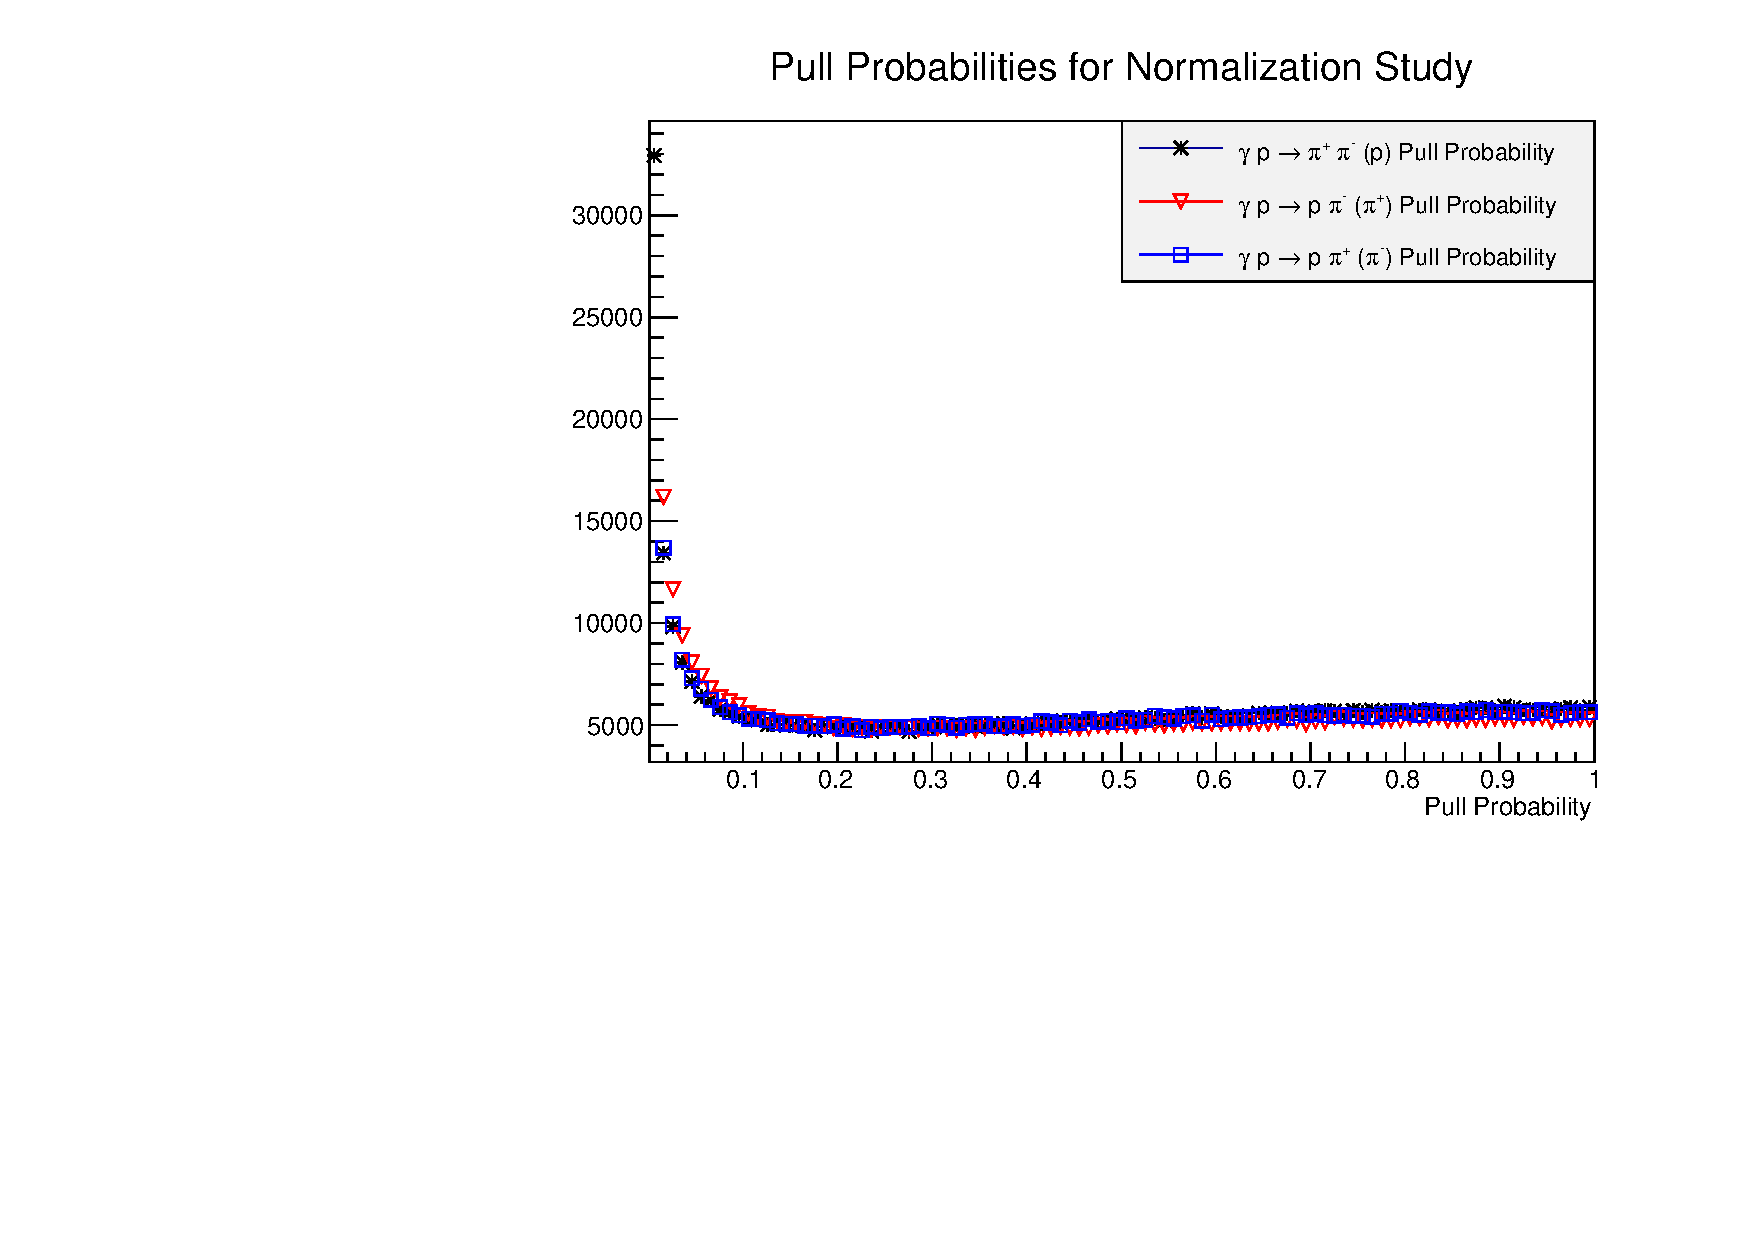
\includegraphics[width=1.1 \figwidth,height=\hfigheight]{\figures/analysis/EFFICIENCY/All_Pull_Eff_Plot.pdf}
\caption[Number of events vs. the pull distribution for the reactions used in the normalization study for data]{\label{fig:eff_pull}Number of events vs. the pull distribution for the reactions used in the normalization study for data.}
\end{center}\end{figure}
\begin{figure}[h!]\begin{center}
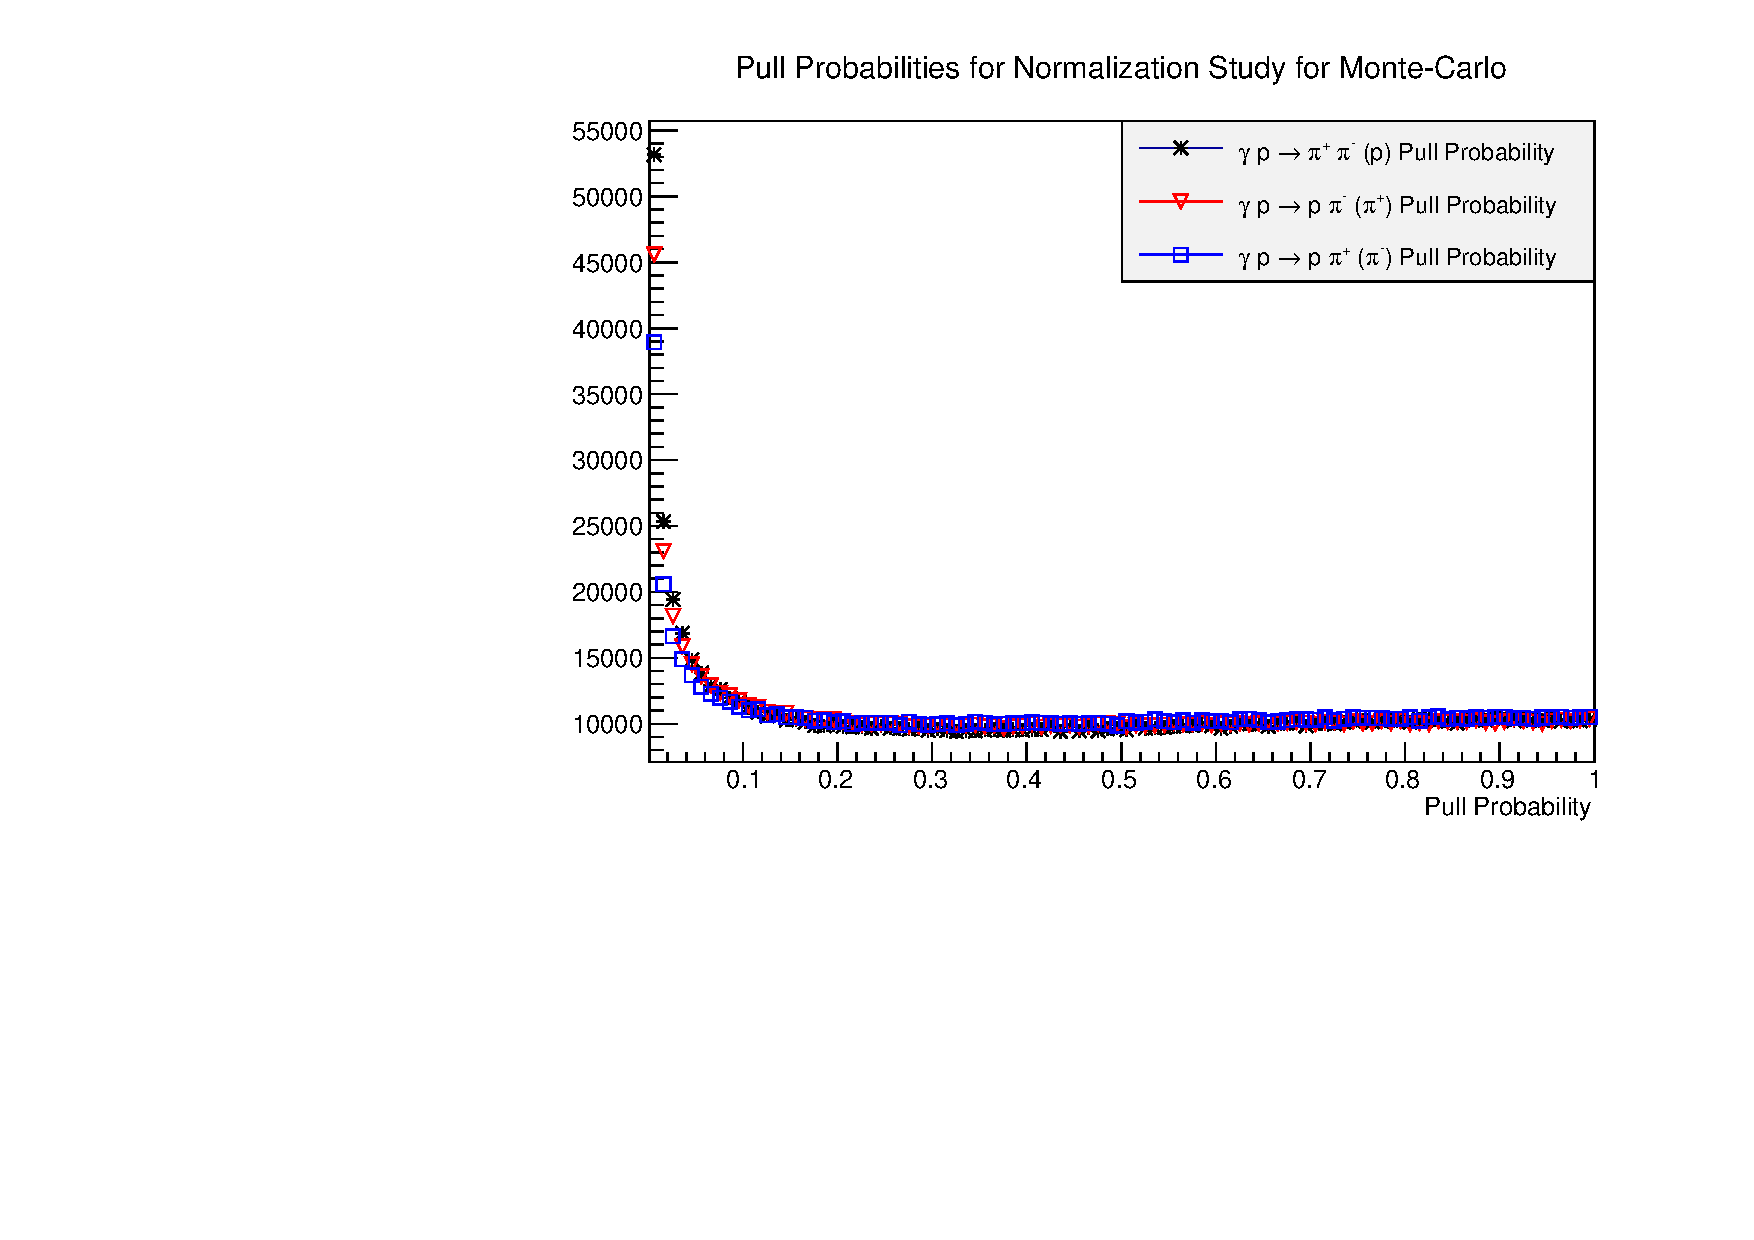
\includegraphics[width=1.1 \figwidth,height=\hfigheight]{\figures/analysis/EFFICIENCY/All_Pull_Eff_PlotMC.pdf}
\caption[Number of events vs. the pull distribution for the reactions used in the normalization study for \abbr{MC}]{\label{fig:eff_pullMC} Number of events vs. the pull distribution for the reactions used in the normalization study for \abbr{MC}.}
\end{center}\end{figure}


The z-vertex of the two needed particles was determined by method of distance of closest approach of the two vectors. The data was then binned for the fitted missing particle according to the z-vertex position, momentum, $\theta \sin\phi$, and $\theta \cos\phi$. The z-vertex and momentum binning used can be seen in Table~\ref{tab:eff_binning}. If the particle to be fit was detected by \abbr{CLAS}, the information was also binned according $z$-vertex, momentum, $\theta \sin\phi$, and $\theta \cos\phi$. However to ensure that the detected particle and the fitted missing particle were the same, the detected particle must have been in the same momentum bin as the fitted missing particle.
%\begin{table}[h!]
%{
%\centering
%\begin{minipage}{\textwidth}
%%\begin{center}
%\begin{singlespacing}
%
%\caption[Binning Used in Efficiency Study]{\label{tab:eff_binning}Binning Used in Efficiency Study \vspace{0.75mm}}
%
%
%\begin{tabular}{c||c|||c||c} \hline
%%%%%%% Title row starts here
%z bins~cm& Momentum bins~GeV & z bins~cm & Momentum bins~GeV \\ \hline
%%%%%%% Row Foo starts here
%$-105 \textless \ z \ \textless -110$ &
%\begin{tabular}{c}
% 0 - 0.5 \\ 0.5 - 0.75 \\ 0.75 - 1 \\ 1 - 1.5 \\ 1.5 - 2  \\2 - 2.5 \\2.5 - 3 \\3 - 5 
%\end{tabular} &
%$-100 \textless \ z \ \textless -105$ &
%\begin{tabular}{c}
% 0 - 0.5 \\ 0.5 - 0.75 \\ 0.75 - 1 \\ 1 - 1.5 \\ 1.5 - 2  \\2 - 2.5 \\2.5 - 3 \\3 - 5 
%\end{tabular} \\ \hline \hline \hline
%%
%%
%z bins~cm& Momentum bins~GeV & z bins~cm & Momentum bins~GeV \\ \hline
%%%%%%% Row Foo starts here
%$-100 \textless \ z \ \textless -95$ &
%\begin{tabular}{c}
% 0 - 0.5 \\ 0.5 - 0.75 \\ 0.75 - 1 \\ 1 - 1.5 \\ 1.5 - 2  \\2 - 2.5 \\2.5 - 3 \\3 - 5 
%\end{tabular} &
%$-95 \textless \ z \ \textless -90$ &
%\begin{tabular}{c}
% 0 - 0.5 \\ 0.5 - 0.75 \\ 0.75 - 1 \\ 1 - 1.5 \\ 1.5 - 2  \\2 - 2.5 \\2.5 - 3 \\3 - 5 
%\end{tabular} \\ \hline \hline \hline
%%
%%
%%
%z bins~cm& Momentum bins~GeV & z bins~cm & Momentum bins~GeV \\ \hline
%%%%%%% Row Foo starts here
%$-90 \textless \ z \ \textless -85$ &
%\begin{tabular}{c}
% 0 - 0.5 \\ 0.5 - 0.75 \\ 0.75 - 1 \\ 1 - 1.5 \\ 1.5 - 2  \\2 - 2.5 \\2.5 - 3 \\3 - 5 
%\end{tabular} &
%$-85 \textless \ z \ \textless -80$ &
%\begin{tabular}{c}
% 0 - 0.5 \\ 0.5 - 0.75 \\ 0.75 - 1 \\ 1 - 1.5 \\ 1.5 - 2  \\2 - 2.5 \\2.5 - 3 \\3 - 5 
%\end{tabular} \\ \hline \hline \hline
%%
%%
%%
%z bins~cm& Momentum bins~GeV & z bins~cm & Momentum bins~GeV \\ \hline
%%%%%%% Row Foo starts here
%$-80 \textless \ z \ \textless -75$ &
%\begin{tabular}{c}
% 0 - 0.5 \\ 0.5 - 0.75 \\ 0.75 - 1 \\ 1 - 1.5 \\ 1.5 - 2  \\2 - 2.5 \\2.5 - 3 \\3 - 5 
%\end{tabular} &
%$-75 \textless \ z \ \textless -70$ &
%\begin{tabular}{c}
% 0 - 0.5 \\ 0.5 - 0.75 \\ 0.75 - 1 \\ 1 - 1.5 \\ 1.5 - 2  \\2 - 2.5 \\2.5 - 3 \\3 - 5 
%\end{tabular} \\ \hline \hline
%
%%Foo &
%%\begin{tabular}{c} 1 \\ 2 \\ 3 \\ 4 \\
%%\end{tabular} &
%%\begin{tabular}{c} 2 \\ 5 \\ 9 \\ 8 \\
%%\end{tabular} \\ \hline \hline
%%
%%%%%%%% Row Bar starts here
%%Bar &
%%\begin{tabular}{c} 1 \\ 2 \\ 3 \\ 4 \\
%%\end{tabular} &
%%\begin{tabular}{c} 31 \\ 23 \\ 16 \\ 42 \\
%%\end{tabular} \\ \hline
%\end{tabular}
%
%
%\end{singlespacing}
%%\end{center}
%\end{minipage}
%}
%\end{table}
%

\begin{table}[h!]
\begin{minipage}{\textwidth}
\begin{center}
\begin{singlespacing}

\caption[Binning Used in Efficiency Study]{\label{tab:eff_binning}Binning Used in Efficiency Study \vspace{0.75mm}}


\begin{tabular}{c||c} \hline
%%%%%% Title row starts here
z bins~[cm] (5~cm \ increments)& Momentum bins~[GeV]  \\ \hline
%%%%%% Row Foo starts here
$-70~\mathrm{cm} \textless \ z \ \textless -110~\mathrm{cm} $  &
\begin{tabular}{c}
 0 - 0.5 \\ 0.5 - 0.75 \\ 0.75 - 1 \\ 1 - 1.5 \\ 1.5 - 2  \\2 - 2.5 \\2.5 - 3 \\3 - 5 
\end{tabular} \\ \hline \hline 

\end{tabular}

\end{singlespacing}
\end{center}
\end{minipage}
\end{table}
\vspace{20pt}
The $\theta \sin\phi$ and $\theta \cos\phi$ binning was chosen to interpret the geometric x and y space the particle travels, independent of momentum and x and y vertex. These $\theta \sin\phi$ and $\theta \cos\phi$ quantities are plotted as x and y variable of a histogram. To better illustrate this interpretation consider a spherical coordinate system where;
\begin{align}
r=\sqrt{x^2 + y^2 + z^2} \\
x = r\sin\theta\cos\phi \\
y = r\sin\theta\sin\phi
\end{align}
therefore,
\begin{align}
\theta \sin\phi = \left(\frac{\theta}{r\sin\theta}\right)y \label{eq:sin1} \\
\theta \cos\phi = \left(\frac{\theta}{r\sin\theta}\right)x \label{eq:sin2} \ .
\end{align}
It can be seen that plotting Eq~\ref{eq:sin2} versus Eq~\ref{eq:sin1} projects $x-y$ space.

For each type of missing particle, we plotted the number of events versus $\theta \sin\phi$ and $\theta \cos\phi$. We then plotted the number of events where the ``missing" particle was detected. The ratio of the number of detected ``missing" particle to the total number of ``missing" particles is the detection efficiency for that bin in $z$-vertex, p, $\theta \sin\phi$ and $\theta \cos\phi$ (see Figs~\ref{fig:eff_prot_data},~\ref{fig:eff_pip_data} and~\ref{fig:eff_pim_data}). This process was repeated for simulated data (see Figs~\ref{fig:eff_prot_MC},~\ref{fig:eff_pip_MC} and~\ref{fig:eff_pim_MC}). The ratio of the simulated efficiency to the measured efficiency for each particle was used to correct the data (see Figs~\ref{fig:toteff_prot},~\ref{fig:toteff_pip} and~\ref{fig:toteff_pim}).
\FloatBarrier
\subsection{\g12 Normalization Results}
It was noticed that the simulation was over-efficient as compared to the data and the ratio of the efficiency of reconstruction should suffice as a correction to the data. Figures~\ref{fig:eff_prot_data},~\ref{fig:eff_pip_data},~\ref{fig:eff_pim_data} depict the efficiency of data reconstruction for the proton $\pi^+$ and $\pi^-$ respectively. Figures~\ref{fig:eff_prot_MC},~\ref{fig:eff_pip_MC},~\ref{fig:eff_pim_MC} depict the efficiency of the simulation reconstruction for the proton $\pi^+$ and $\pi^-$ respectively. Figures~\ref{fig:toteff_prot},~\ref{fig:toteff_pip},~\ref{fig:toteff_pim} depict the over-efficiency of the simulation to data reconstruction for the proton $\pi^+$ and $\pi^-$ respectively.
% % %PROTON
\begin{figure}[h!]\begin{center}
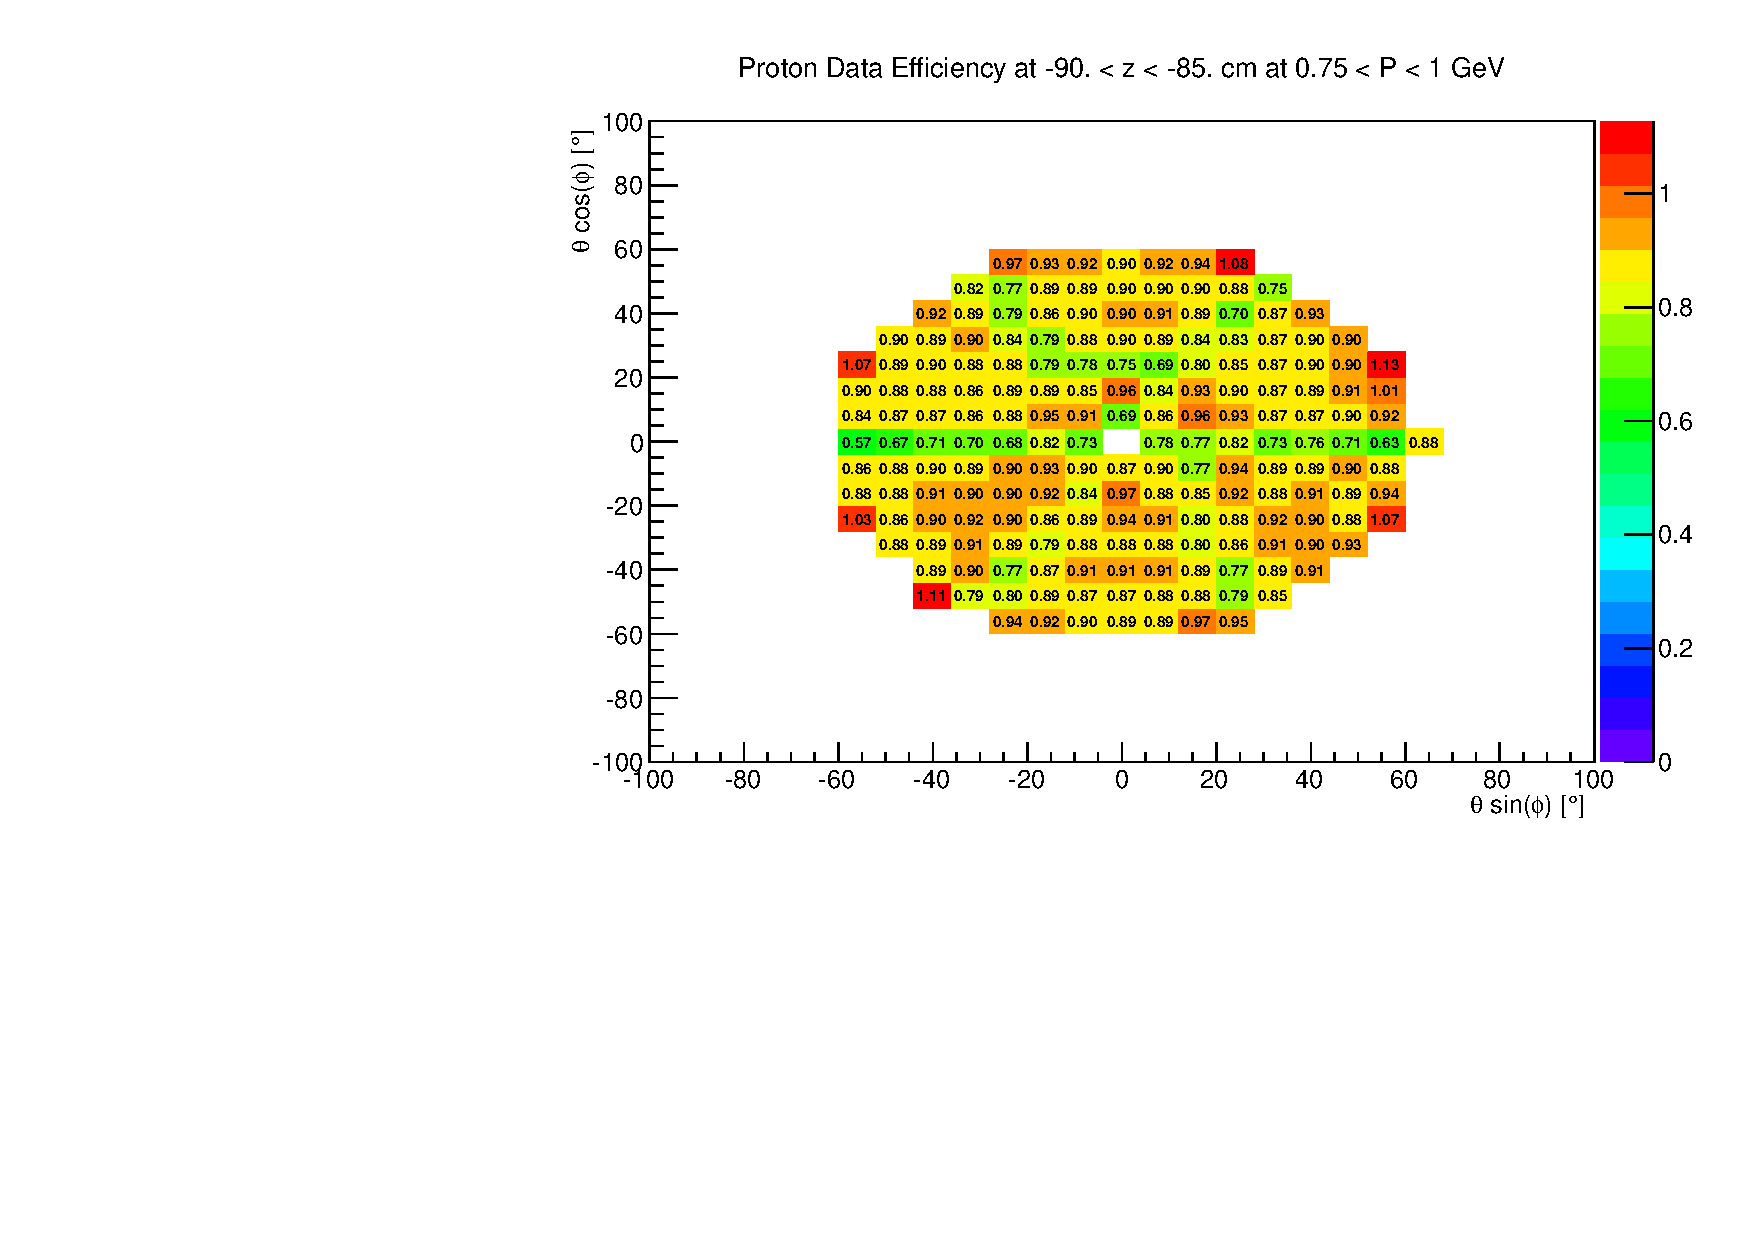
\includegraphics[width=1.1 \figwidth,height=\hfigheight]{\figures/analysis/EFFICIENCY/Prot_Thesis_EffData_Plot.pdf}
\caption[$\theta \cos\phi$ vs. $\theta \sin\phi$ plot showing the efficiency of detecting the proton with z-vertex $-90\textless z\textless-85$~cm and momentum $0.75\textless p \textless 1$~GeV from a 2 charged track reaction using \abbr{CLAS} detection for \g12]{\label{fig:eff_prot_data} $\theta \cos\phi$ vs. $\theta \sin\phi$ plot showing the efficiency of detecting the proton with z-vertex $-90\textless z\textless-85$~cm and momentum $0.75\textless p \textless 1$~GeV from a 2 charged track reaction using \abbr{CLAS} detection for \g12.}
\end{center}\end{figure}
%
\begin{figure}[h!]\begin{center}
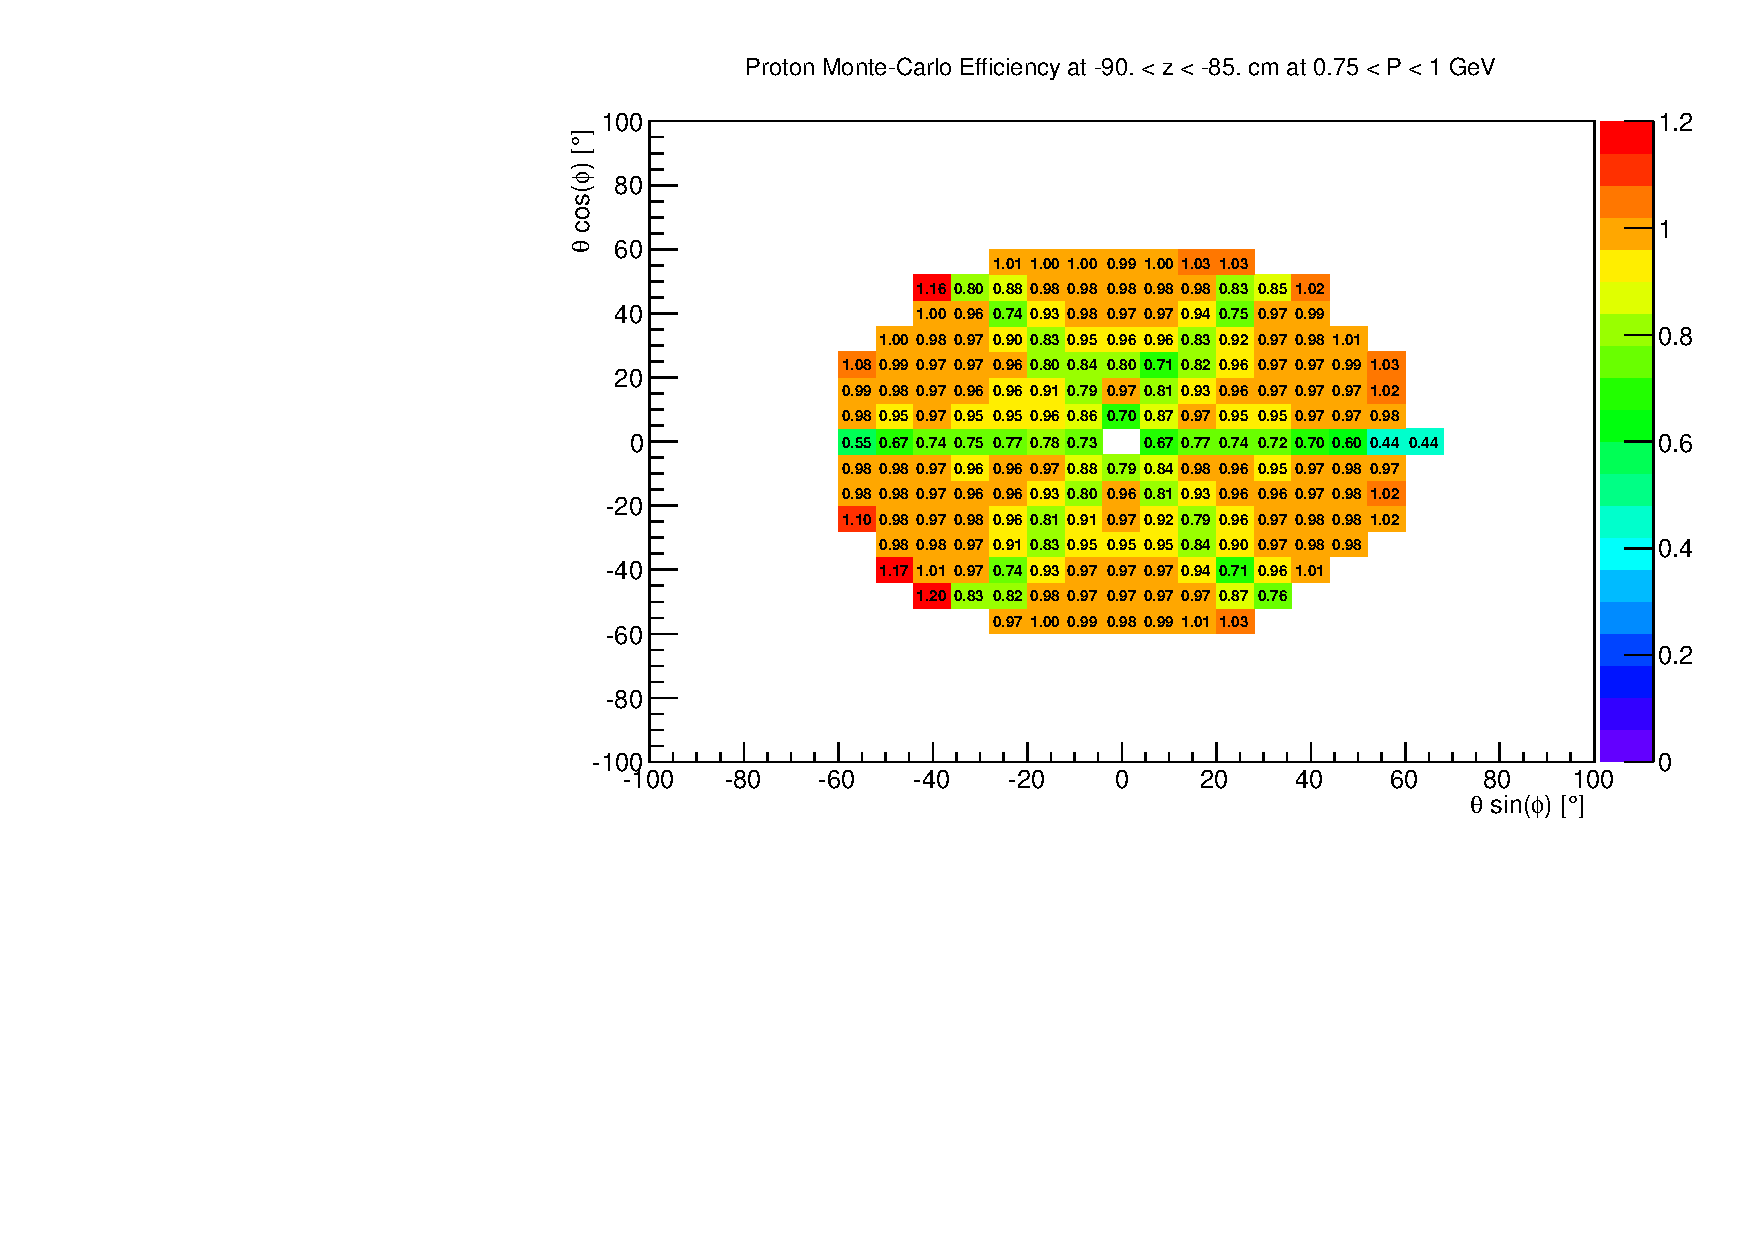
\includegraphics[width=1.1 \figwidth,height=\hfigheight]{\figures/analysis/EFFICIENCY/Prot_Thesis_EffMC_Plot.pdf}
\caption[$\theta \cos\phi$ vs. $\theta \sin\phi$ plot showing the efficiency of reconstructing the proton with z-vertex $-90\textless z\textless-85$~cm and momentum $0.75\textless p \textless 1$~GeV from a 2 charged track reaction using \abbr{CLAS} Monte-Carlo for \g12]{\label{fig:eff_prot_MC} $\theta \cos\phi$ vs. $\theta \sin\phi$ plot showing the efficiency of reconstructing the proton with z-vertex $-90\textless z\textless-85$~cm and momentum $0.75\textless p \textless 1$~GeV from a 2 charged track reaction using \abbr{CLAS} Monte-Carlo for \g12.}
\end{center}\end{figure}
%
\begin{figure}[h!]\begin{center}
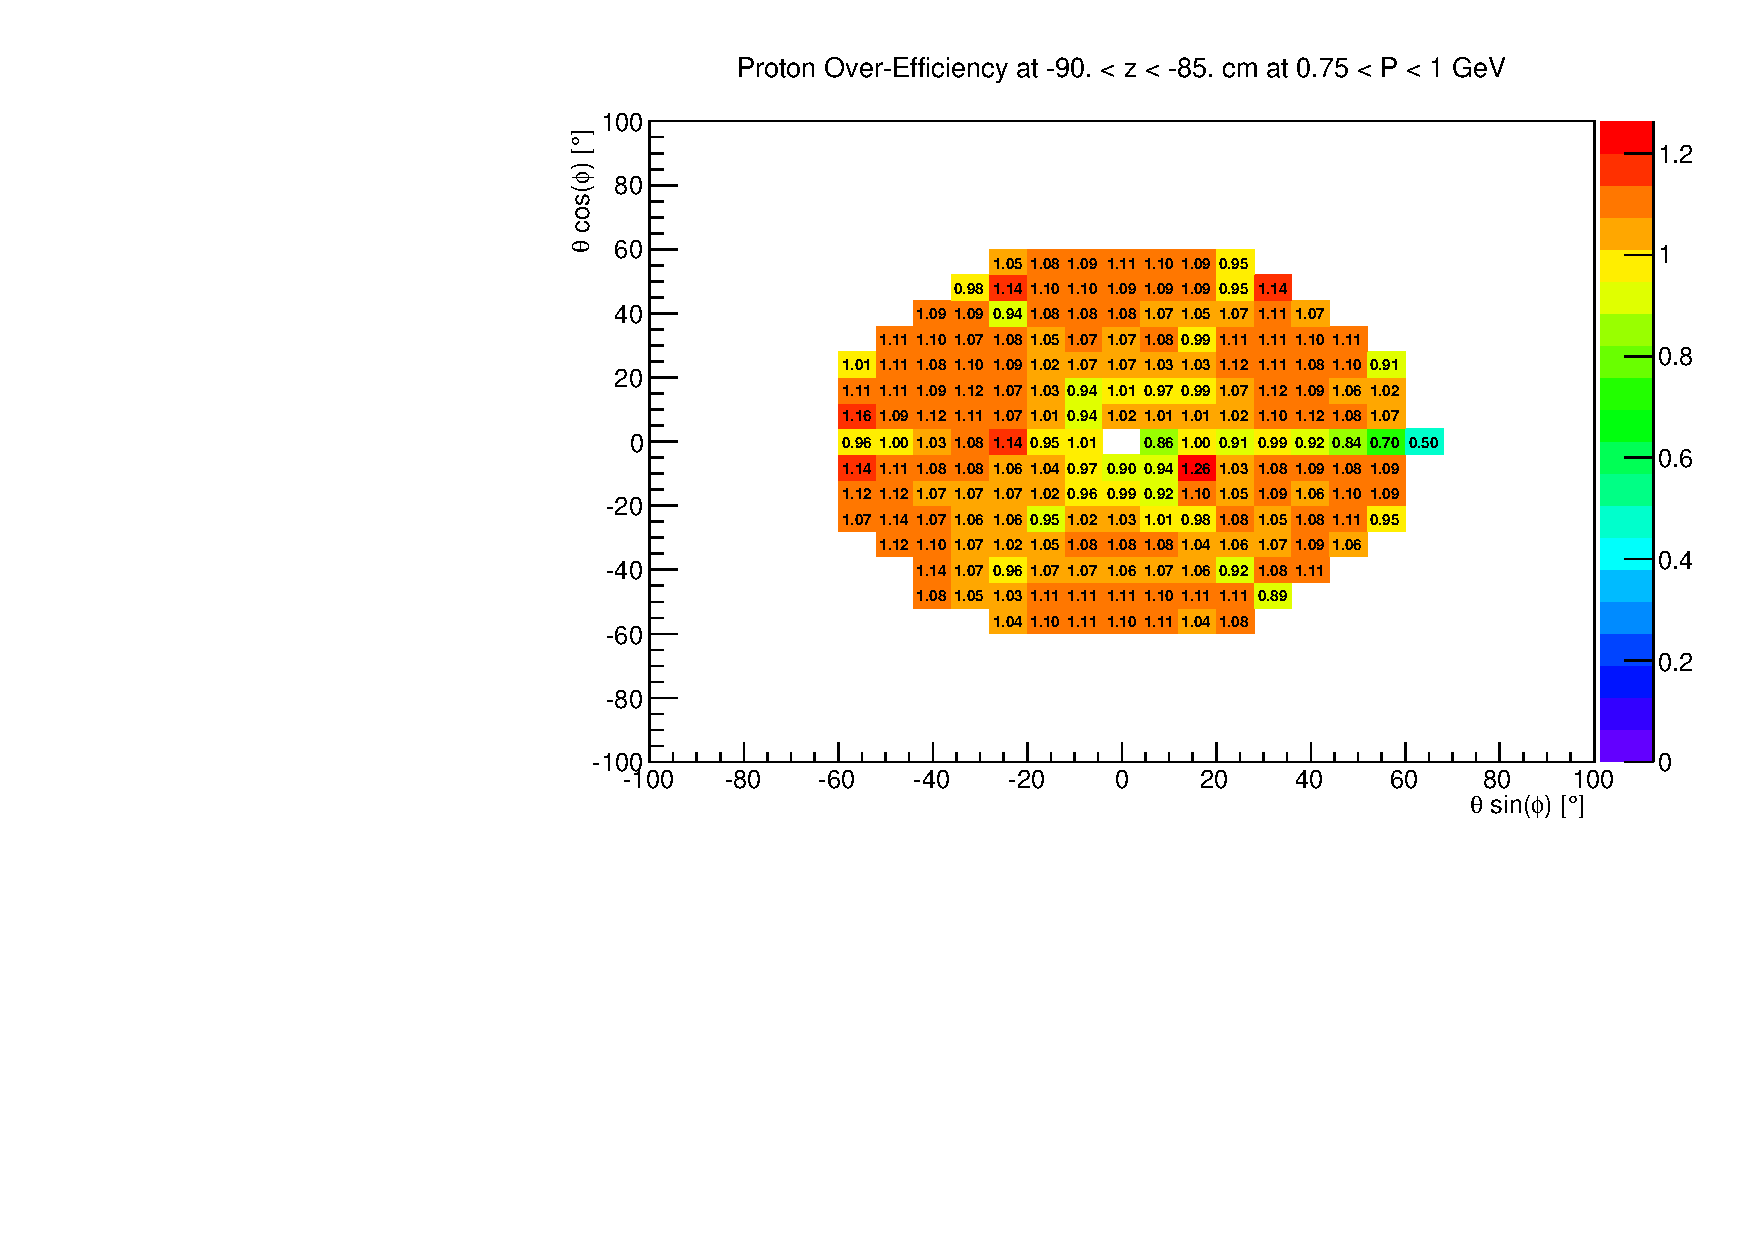
\includegraphics[width=1.1 \figwidth,height=\hfigheight]{\figures/analysis/EFFICIENCY/Prot_Thesis_TotEff_Plot.pdf}
\caption[$\theta \cos\phi$ vs. $\theta \sin\phi$ plot showing the over-efficiency of simulating the proton with z-vertex $-90\textless z\textless-85$~cm and momentum $0.75\textless p \textless 1$~GeV from a 2 charged track reaction]{\label{fig:toteff_prot} $\theta \cos\phi$ vs. $\theta \sin\phi$ plot showing the over-efficiency of simulating the proton with z-vertex $-90\textless z\textless-85$~cm and momentum $0.75\textless p \textless 1$~GeV from a 2 charged track reaction.}
\end{center}\end{figure}
% % %PIP
\begin{figure}[h!]\begin{center}
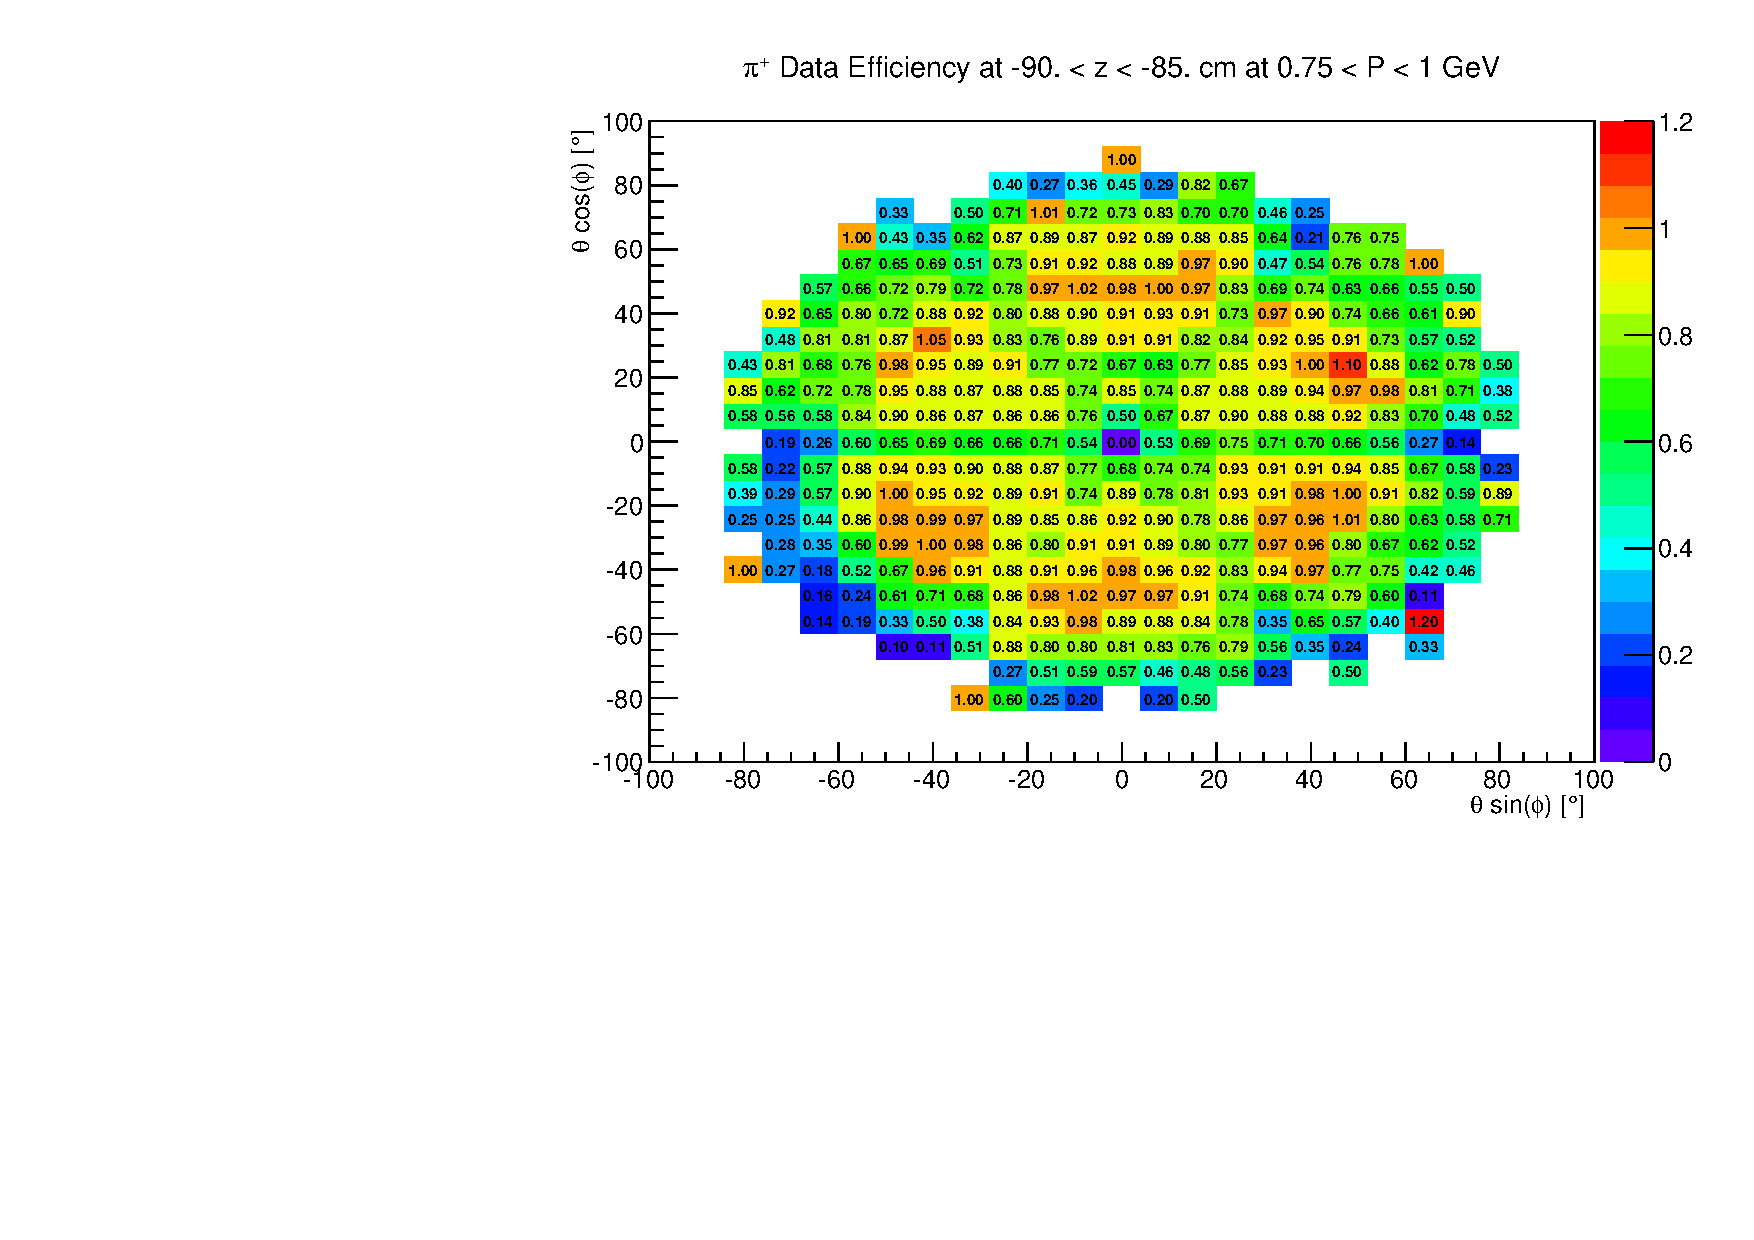
\includegraphics[width=1.1 \figwidth,height=\hfigheight]{\figures/analysis/EFFICIENCY/Pip_Thesis_EffData_Plot.pdf}
\caption[$\theta \cos\phi$ vs. $\theta \sin\phi$ plot showing the efficiency of detecting the $\pi^+$ with z-vertex $-90\textless z\textless-85$~cm and momentum $0.75\textless p \textless 1$~GeV from a 2 charged track reaction using \abbr{CLAS} detection for \g12]{\label{fig:eff_pip_data} $\theta \cos\phi$ vs. $\theta \sin\phi$ plot showing the efficiency of detecting the $\pi^+$ with z-vertex $-90\textless z\textless-85$~cm and momentum $0.75\textless p \textless 1$~GeV from a 2 charged track reaction using \abbr{CLAS} detection for \g12.}
\end{center}\end{figure}
%
\begin{figure}[h!]\begin{center}
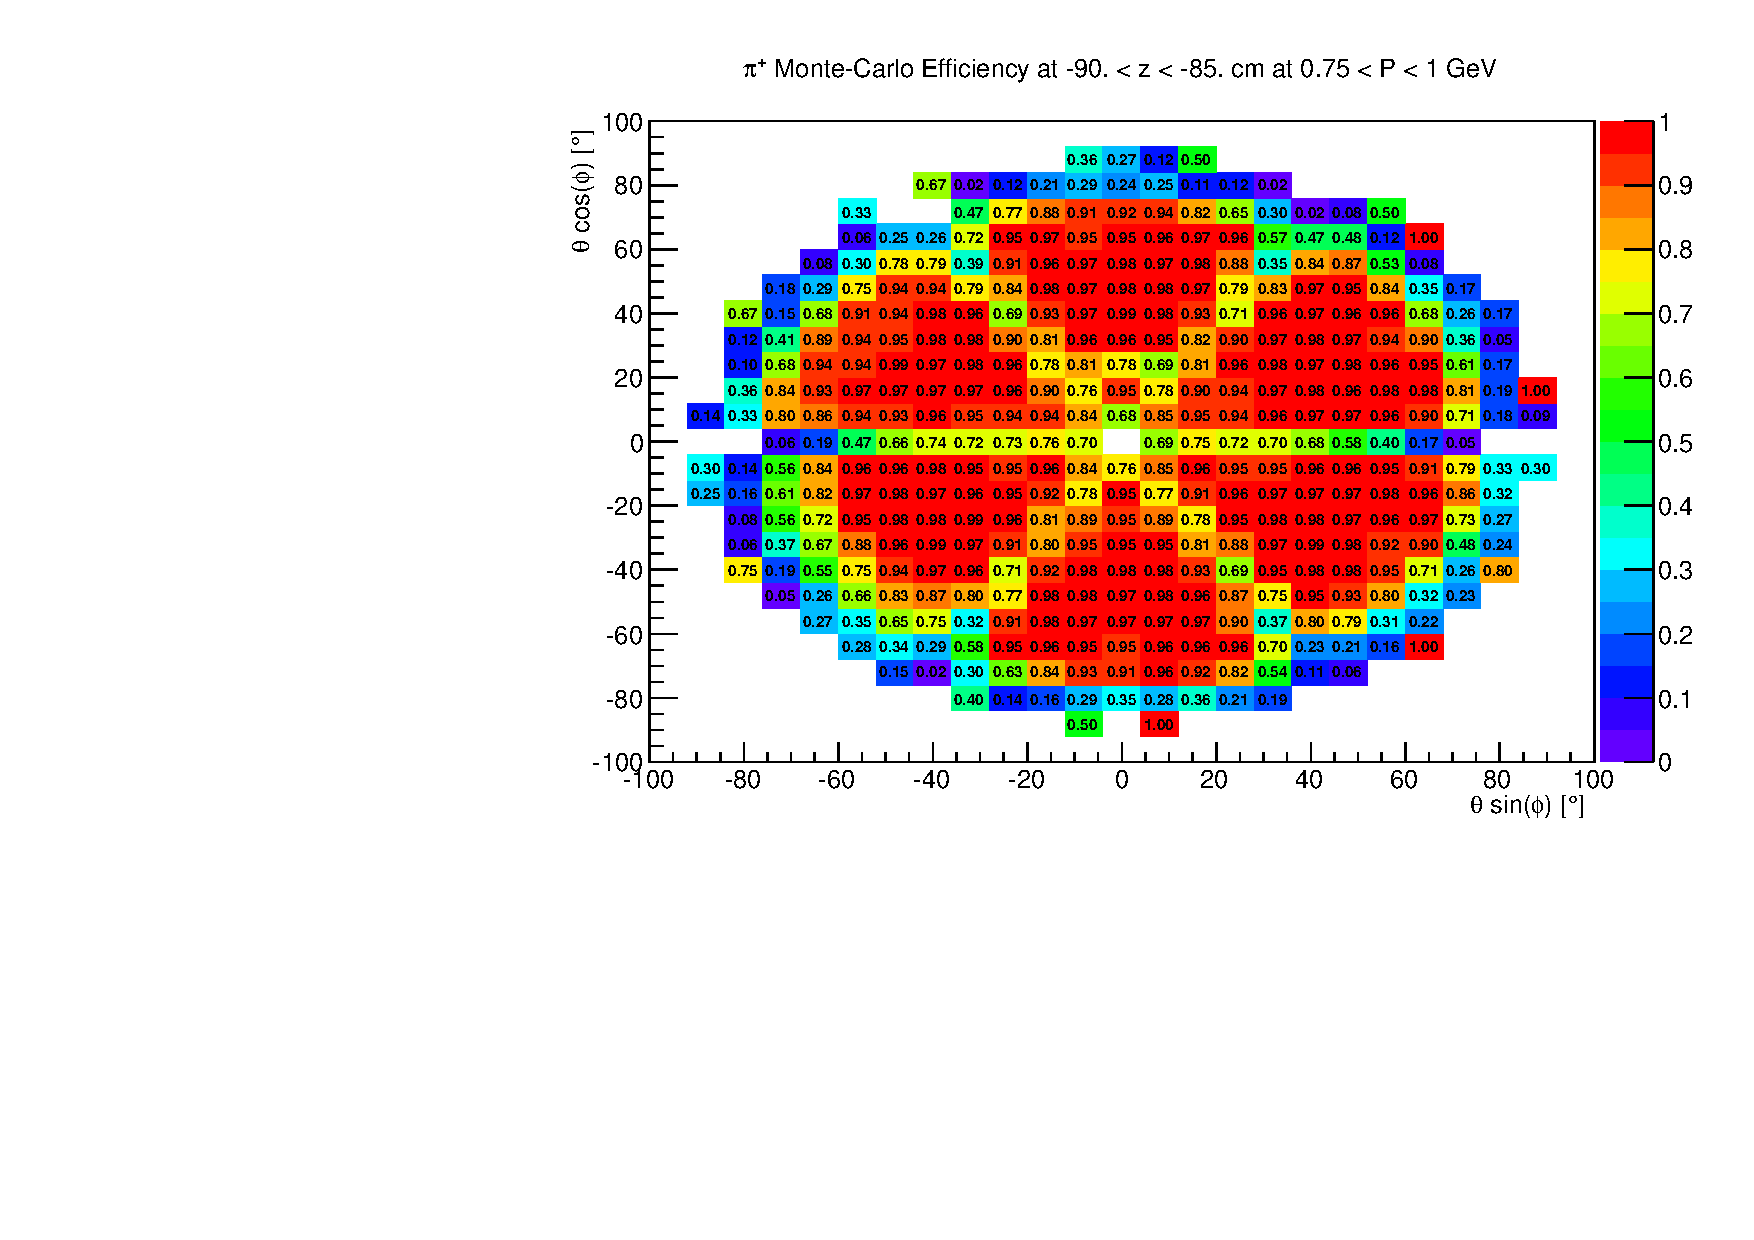
\includegraphics[width=1.1 \figwidth,height=\hfigheight]{\figures/analysis/EFFICIENCY/Pip_Thesis_EffMC_Plot.pdf}
\caption[$\theta \cos\phi$ vs. $\theta \sin\phi$ plot showing the efficiency of reconstructing the $\pi^+$ with z-vertex $-90\textless z\textless-85$~cm and momentum $0.75\textless p \textless 1$~GeV from a 2 charged track reaction using \abbr{CLAS} Monte-Carlo for \g12]{\label{fig:eff_pip_MC} $\theta \cos\phi$ vs. $\theta \sin\phi$ plot showing the efficiency of reconstructing the $\pi^+$ with z-vertex $-90\textless z\textless-85$~cm and momentum $0.75\textless p \textless 1$~GeV from a 2 charged track reaction using \abbr{CLAS} Monte-Carlo for \g12.}
\end{center}\end{figure}
%
\begin{figure}[h!]\begin{center}
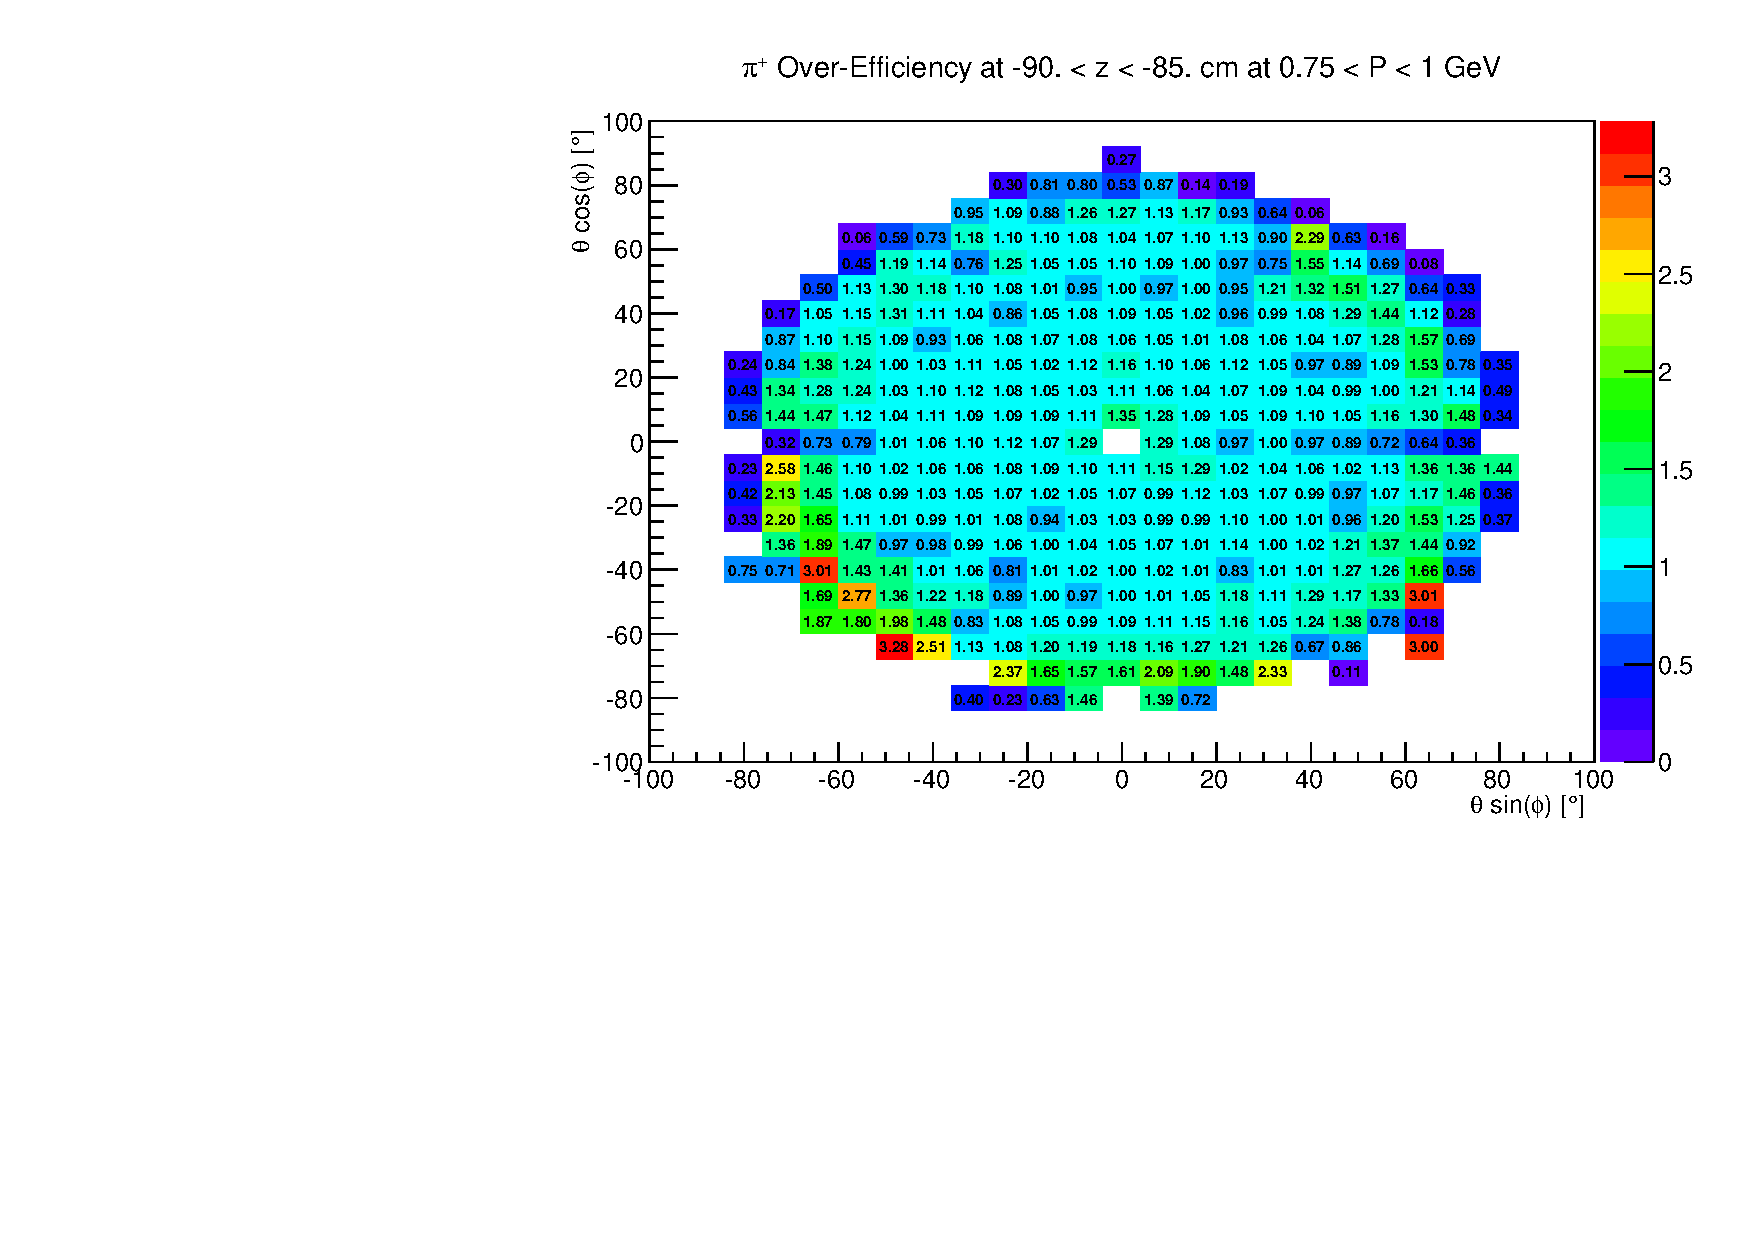
\includegraphics[width=1.1 \figwidth,height=\hfigheight]{\figures/analysis/EFFICIENCY/Pip_Thesis_TotEff_Plot.pdf}
\caption[$\theta \cos\phi$ vs. $\theta \sin\phi$ plot showing the over-efficiency of simulating the $\pi^+$ with z-vertex $-90\textless z\textless-85$~cm and momentum $0.75\textless p \textless 1$~GeV from a 2 charged track reaction]{\label{fig:toteff_pip} $\theta \cos\phi$ vs. $\theta \sin\phi$ plot showing the over-efficiency of simulating the $\pi^+$ with z-vertex $-90\textless z\textless-85$~cm and momentum $0.75\textless p \textless 1$~GeV from a 2 charged track reaction.}
\end{center}\end{figure}
% % %PIM
\begin{figure}[h!]\begin{center}
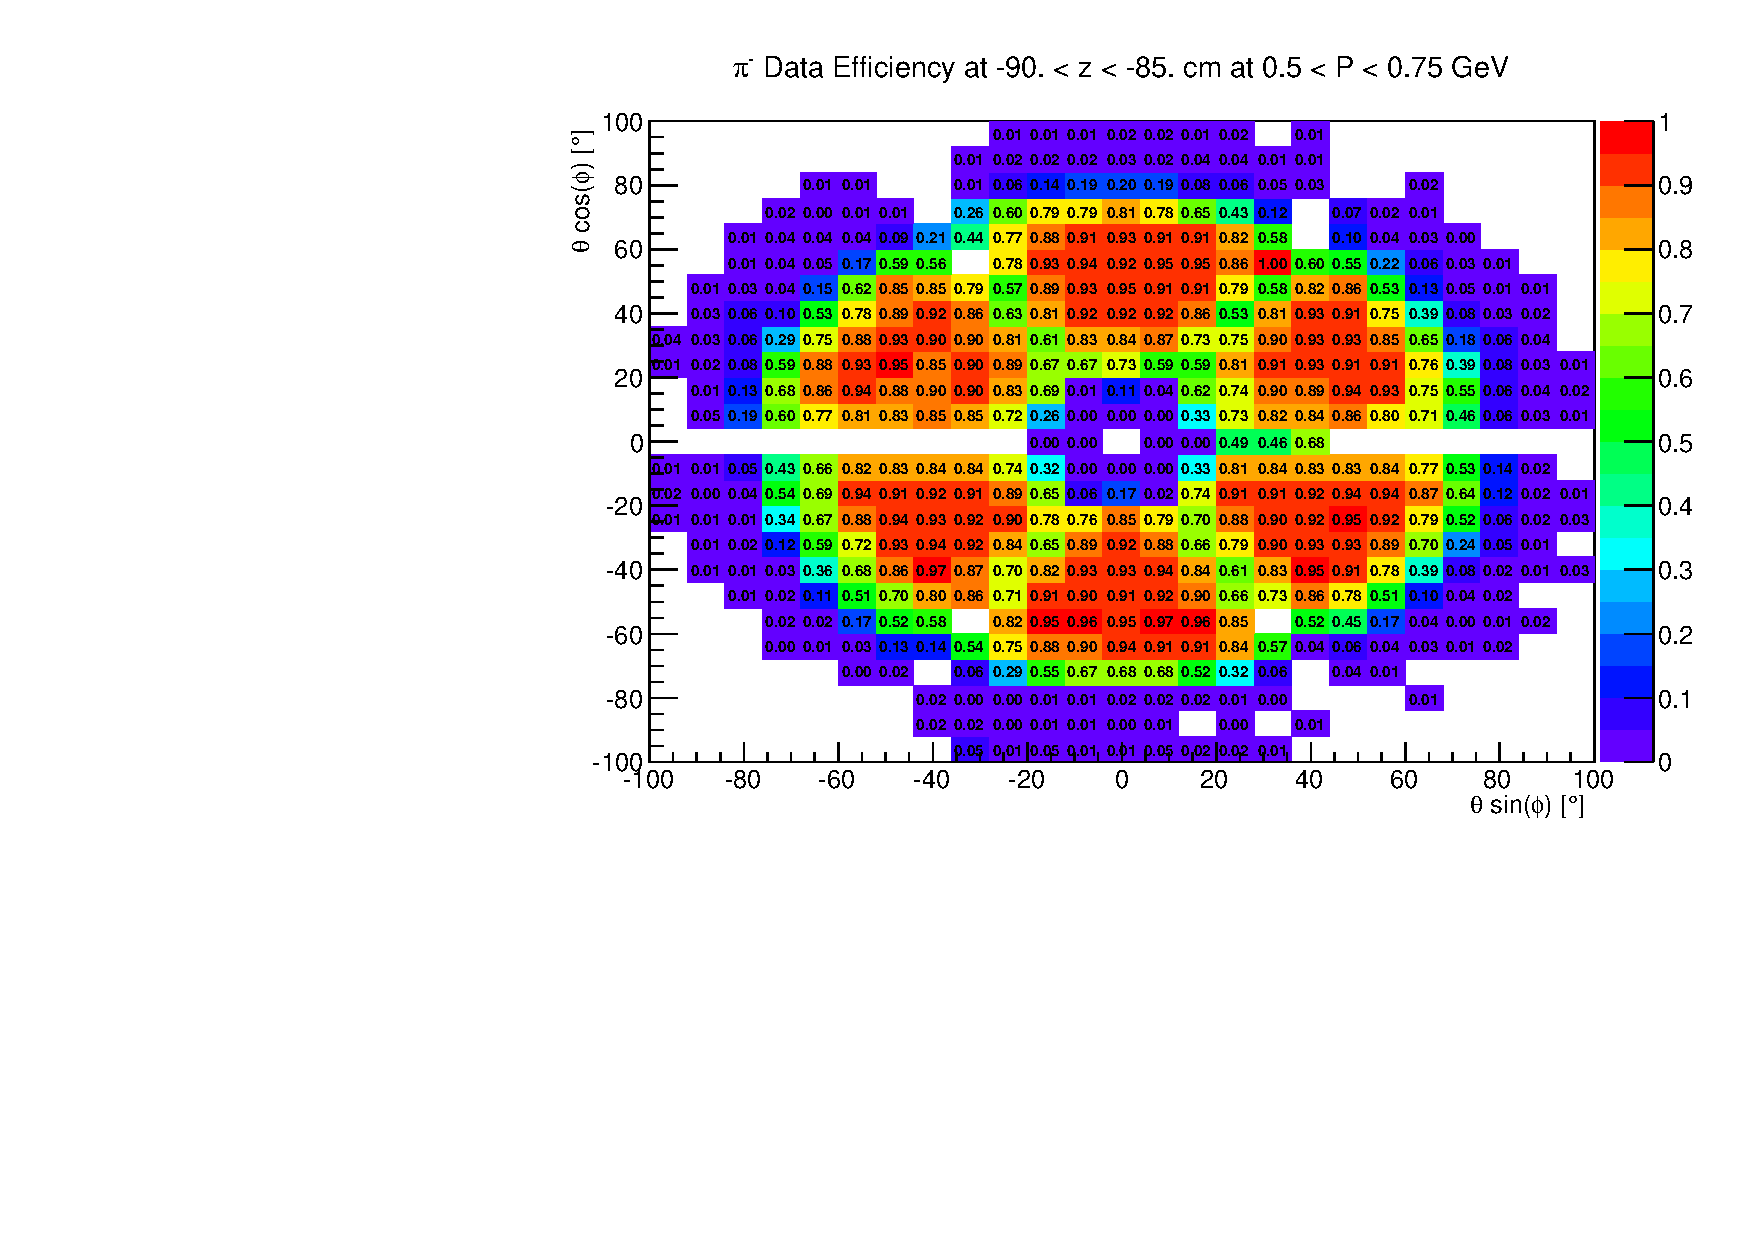
\includegraphics[width=1.1 \figwidth,height=\hfigheight]{\figures/analysis/EFFICIENCY/Pim_Thesis_EffData_Plot.pdf}
\caption[$\theta \cos\phi$ vs. $\theta \sin\phi$ plot showing the efficiency of detecting the $\pi^-$ with z-vertex $-90\textless z\textless-85$~cm and momentum $0.75\textless p \textless 1$~GeV from a 2 charged track reaction using \abbr{CLAS} detection for \g12]{\label{fig:eff_pim_data} $\theta \cos\phi$ vs. $\theta \sin\phi$ plot showing the efficiency of detecting the $\pi^-$ with z-vertex $-90\textless z\textless-85$~cm and momentum $0.75\textless p \textless 1$~GeV from a 2 charged track reaction using \abbr{CLAS} detection for \g12.}
\end{center}\end{figure}
%
\begin{figure}[h!]\begin{center}
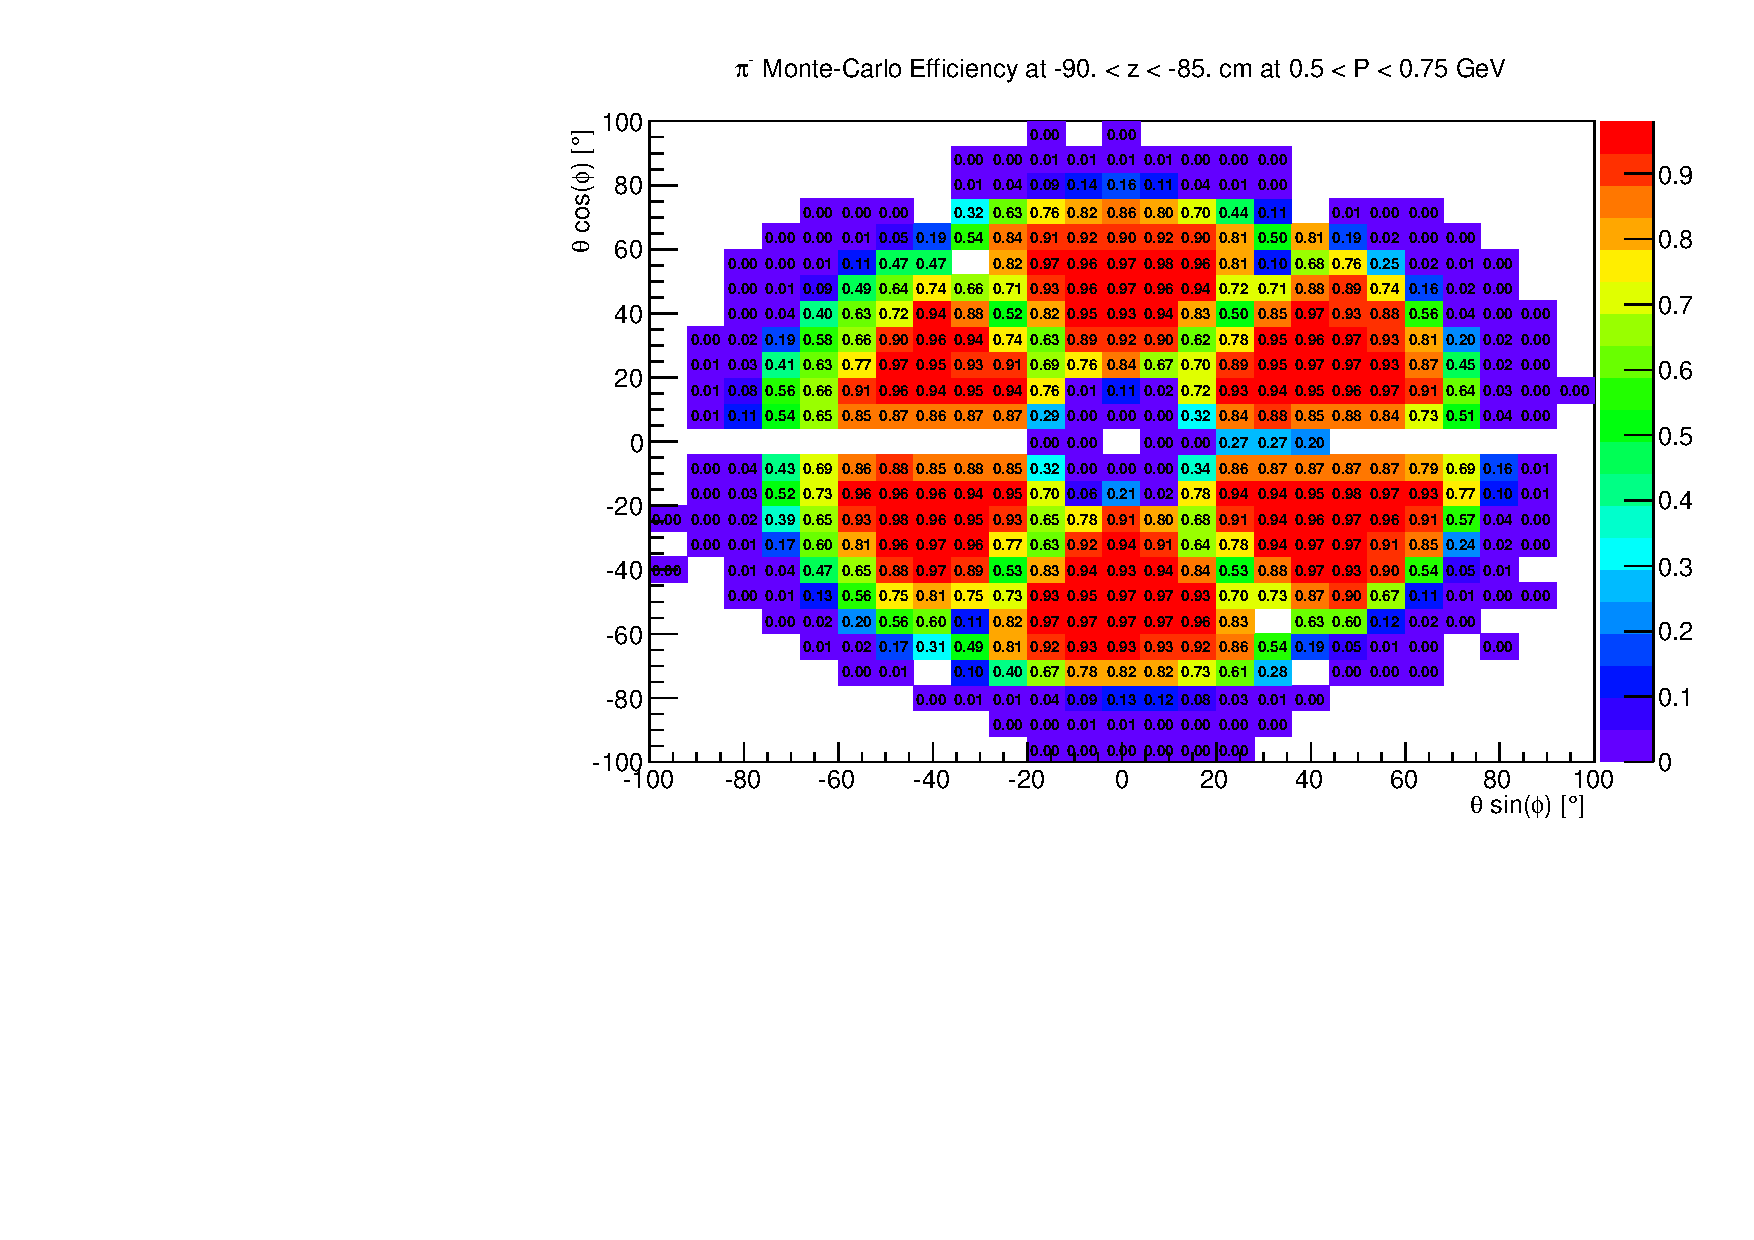
\includegraphics[width=1.1 \figwidth,height=\hfigheight]{\figures/analysis/EFFICIENCY/Pim_Thesis_EffMC_Plot.pdf}
\caption[$\theta \cos\phi$ vs. $\theta \sin\phi$ plot showing the efficiency of reconstructing the $\pi^-$ with z-vertex $-90\textless z\textless-85$~cm and momentum $0.75\textless p \textless 1$~GeV from a 2 charged track reaction using \abbr{CLAS} Monte-Carlo for \g12]{\label{fig:eff_pim_MC} $\theta \cos\phi$ vs. $\theta \sin\phi$ plot showing the efficiency of reconstructing the $\pi^-$ with z-vertex $-90\textless z\textless-85$~cm and momentum $0.75\textless p \textless 1$~GeV from a 2 charged track reaction using \abbr{CLAS} Monte-Carlo for \g12.}
\end{center}\end{figure}
%
\begin{figure}[h!]\begin{center}
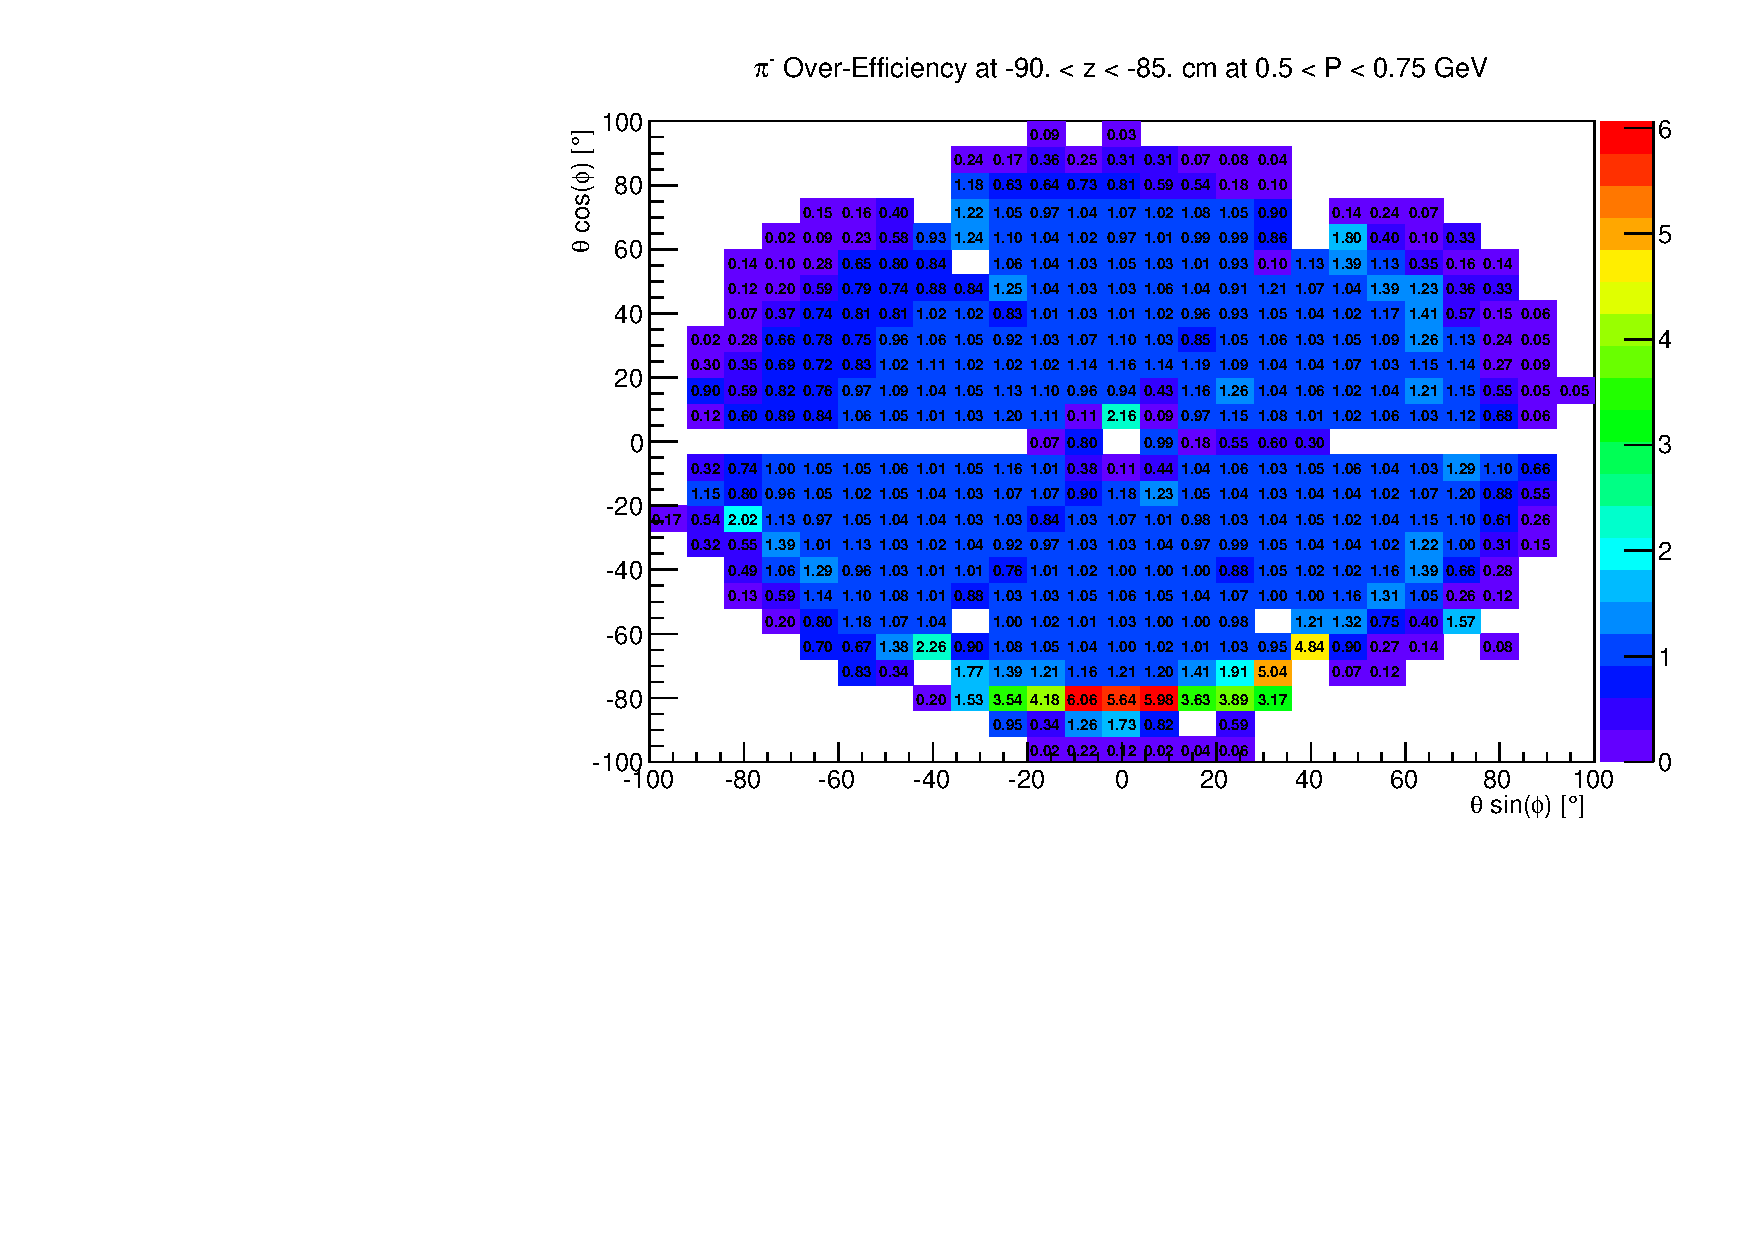
\includegraphics[width=1.1 \figwidth,height=\hfigheight]{\figures/analysis/EFFICIENCY/Pim_Thesis_TotEff_Plot.pdf}
\caption[$\theta \cos\phi$ vs. $\theta \sin\phi$ plot showing the over-efficiency of simulating the $\pi^-$ with z-vertex $-90\textless z\textless-85$~cm and momentum $0.75\textless p \textless 1$~GeV from a 2 charged track reaction]{\label{fig:toteff_pim} $\theta \cos\phi$ vs. $\theta \sin\phi$ plot showing the over-efficiency of simulating the $\pi^-$ with z-vertex $-90\textless z\textless-85$~cm and momentum $0.75\textless p \textless 1$~GeV from a 2 charged track reaction.}
\end{center}\end{figure}
%
The total over-efficiency was calculated as the product of each track's over-efficiency, i.e.,
\begin{align}\label{eq:eff_tot}
\epsilon = \epsilon_{proton}\cdot\epsilon_{\pi^+}\cdot\epsilon_{\pi^-}.
\end{align}
The value of $\epsilon$ from eq.~\ref{eq:eff_tot} is the same quantity used in the cross-section calculation in eq.~\ref{eq:xsection1}.
\FloatBarrier
%
\subsection{Normalization Comparison}
To validate the \g12 normalization results, the \g12 $\pi^0$ differential cross-section was calculated using the \G11 global normalization factor and then compared to the \g12 $\pi^0$ differential cross-section using the \g12 normalization procedure results. It is shown in Fig.~\ref{fig:toteff_compareI} and Fig.~\ref{fig:toteff_compareII} that the 2 methods agree with one another except for the very forward regions of $\cos\theta^{\pi^0}_{C.M.}$, where the cross-section using the dynamic normalization is larger than the cross-section measured with the \G11 global normalization, however the larger cross-sections at forward $\cos\theta^{\pi^0}_{C.M.}$ agree very well with the past results of~\cite{ELSA11}.

\begin{figure}[h!]\begin{center}
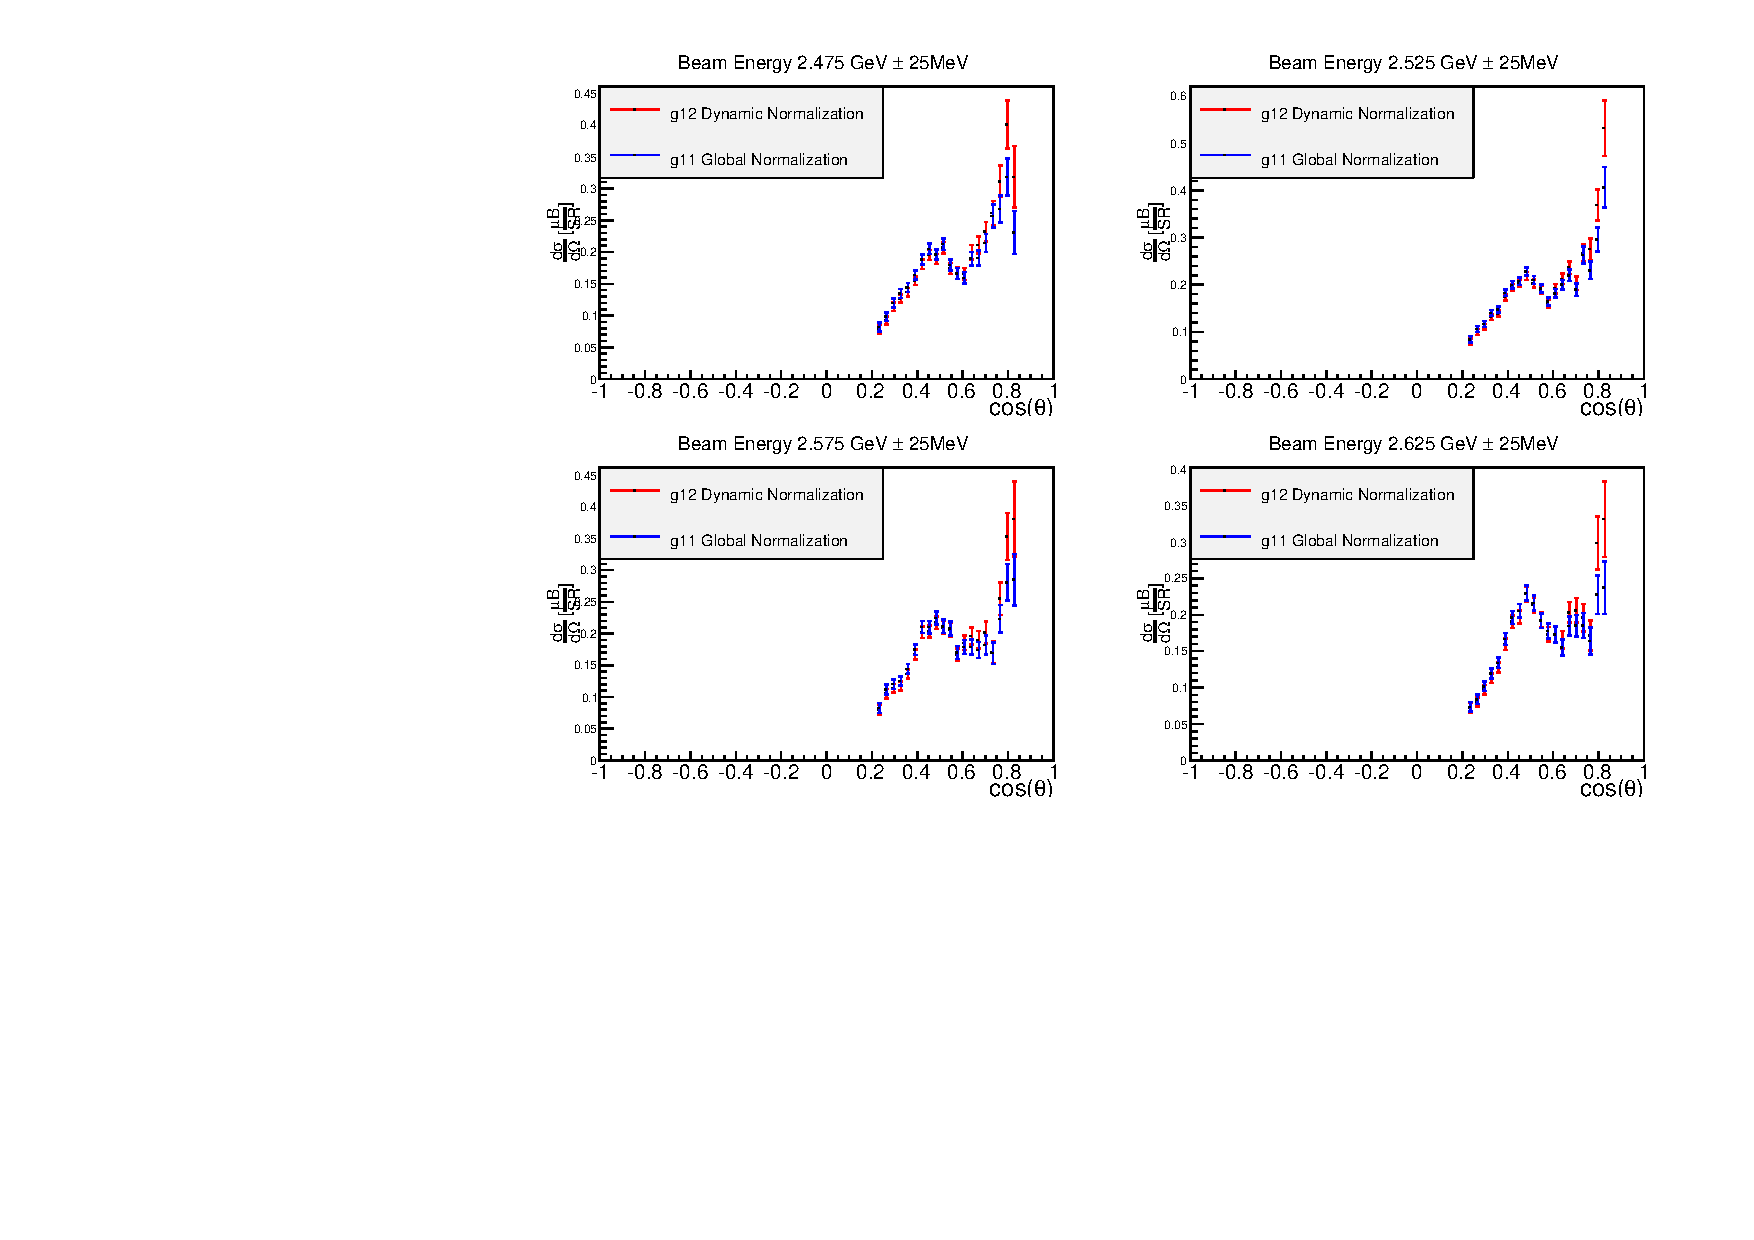
\includegraphics[width=1.1 \figwidth,height=\hfigheight]{\figures/analysis/EFFICIENCY/G12_XSection_Normaization_Compare_thesisI.pdf}
\caption[$\frac{d \sigma}{d \Omega}$ vs. $\cos \theta$ plot showing the \g12 \piz differential cross-section when the \G11 global normalization is used (blue) and when the \g12 dynamic normalization is used (red) for various bins of beam energy inside lepton trigger acceptance]{\label{fig:toteff_compareI} $\frac{d \sigma}{d \Omega}$ vs. $\cos \theta$ plot showing the \g12 \piz differential cross-section when the \G11 global normalization is used (blue) and when the \g12 dynamic normalization is used (red) for various bins of beam energy inside lepton trigger acceptance.}
\end{center}\end{figure}

\begin{figure}[h!]\begin{center}
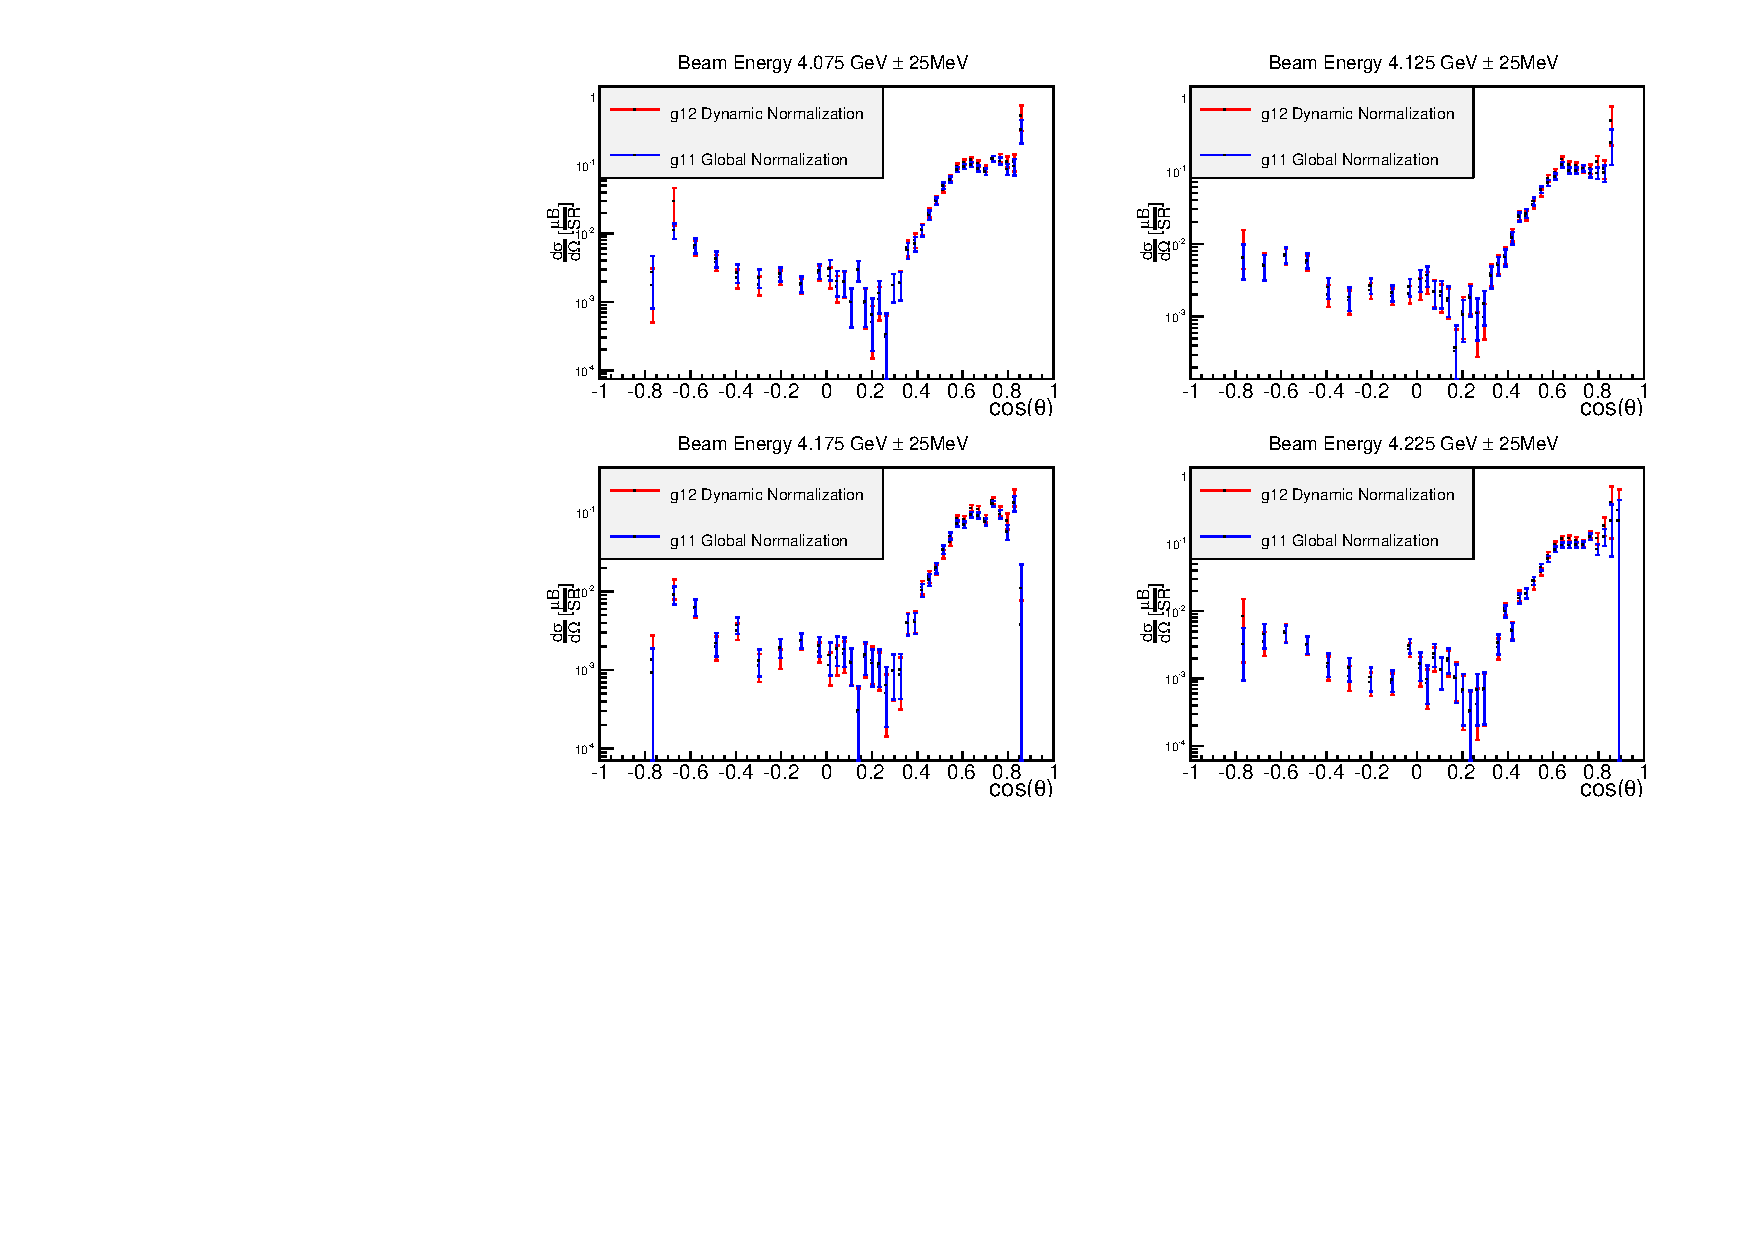
\includegraphics[width=1.1 \figwidth,height=\hfigheight]{\figures/analysis/EFFICIENCY/G12_XSection_Normaization_Compare_thesisII.pdf}
\caption[$\frac{d \sigma}{d \Omega}$ vs. $\cos \theta$ plot showing the \g12 \piz differential cross-section when the \G11 global normalization is used (blue) and when the \g12 dynamic normalization is used (red) for various bins of beam energy above \abbr{MORB} threshold]{\label{fig:toteff_compareII} $\frac{d \sigma}{d \Omega}$ vs. $\cos \theta$ plot showing the \g12 \piz differential cross-section when the \G11 global normalization is used (blue) and when the \g12 dynamic normalization is used (red) for various bins of beam energy above \abbr{MORB} threshold.}
\end{center}\end{figure}

\FloatBarrier

\subsection{Normalization Uncertainties}
The statistical uncertainties of the normalization correction was minimized by ensuring that the statistical sample of the data and \abbr{MC} was sufficient in each bin of $z$-vertex, momentum, $\theta \sin\phi$ and $\theta \cos\phi$. The maximum statistical uncertainty was 0.01\%. The systematic uncertainties of the normalization correction was not calculated, but it is intended to be.